\documentclass[compress,red]{beamer}
\mode<presentation>
\setbeamertemplate{navigation symbols}{}

\usetheme{Warsaw}


%\hypersetup{pdfpagemode=FullScreen} % makes your presentation go automatically to full screen

% define your own colors:
\definecolor{Red}{rgb}{1,0,0}
\definecolor{Blue}{rgb}{0,0,1}
\definecolor{Green}{rgb}{0,1,0}
\definecolor{magenta}{rgb}{1,0,.6}
\definecolor{lightblue}{rgb}{0,.5,1}
\definecolor{lightpurple}{rgb}{.6,.4,1}
\definecolor{gold}{rgb}{.6,.5,0}
\definecolor{orange}{rgb}{1,0.4,0}
\definecolor{hotpink}{rgb}{1,0,0.5}
\definecolor{newcolor2}{rgb}{.5,.3,.5}
\definecolor{newcolor}{rgb}{0,.3,1}
\definecolor{newcolor3}{rgb}{1,0,.35}
\definecolor{darkgreen1}{rgb}{0, .35, 0}
\definecolor{darkgreen}{rgb}{0, .6, 0}
\definecolor{darkred}{rgb}{.75,0,0}

\xdefinecolor{olive}{cmyk}{0.64,0,0.95,0.4}
\xdefinecolor{purpleish}{cmyk}{0.75,0.75,0,0}


\useoutertheme[subsection=false]{smoothbars}


% include packages
\usepackage{subfigure}
\usepackage{multicol}
\usepackage{amsmath}
\usepackage{epsfig}
\usepackage{graphicx}
\usepackage[all,knot]{xy}
\xyoption{arc}
\usepackage{url}
\usepackage{multimedia}
\usepackage{hyperref}
\usepackage{helvet}
\usepackage[polish,english]{babel}
\usepackage[utf8]{inputenc}
\usepackage{multirow}

\graphicspath{ {../../figures/} }
%%%%%%%%%%%%5
%\usepackage{geometry}
%\geometry{verbose,letterpaper}
%\usepackage{movie15}
%\usepackage{hyperref}
%%%%%%%

% greetings, introduce yourself


%  \includegraphics[height=5cm]{fig/WRlogo.ps}


\title[White Rabbit \hspace{2em}\insertframenumber/ \inserttotalframenumber]
{White Rabbit\\ a PTP Application for Robust Sub-nanosecond Synchronization}

\institute{
Hardware and Timing Section\\
The European Organization for Nuclear Research (CERN)\\
Geneve, Switzerland.
}
\author{
Maciej Lipi\'{n}ski %, T.W\l{}ostowski, J.Serrano, P.Alvarez
}
\date{September 14, 2011}



% \institute%[Universities of Somewhere and Elsewhere] % (optional, but mostly needed)
% {
%   \begin{center}
%     BE-CO-HT\\
%     CERN, Geneva,\\
%     Switzerland\\
%   \end{center}
% }

\pgfdeclareimage[height=0.6cm]{wr-logo}{logo/WRlogo.ps}
\logo{\pgfuseimage{wr-logo}}
\AtBeginSection[]
% {
%   \begin{frame}<beamer>{Outline}
%     \tableofcontents[currentsection]
%   \end{frame}
% }

\begin{document}

\frame{\titlepage}
%%%%%%%%%%%%%%%%%%%%%%%%%%%%%%%%%%%%%%%%%%%%%%%%%%%%%%%%%%%%%%%%%%%%%%%%%%%%%%%%%%%%%%%%%%%%%%%%%%%%
\begin{frame}<beamer>{Outline}

    \tableofcontents %[currentsection]

\end{frame}
%%%%%%%%%%%%%%%%%%%%%%%%%%%%%%%%%%%%%%%%%%%%%%%%%%%%%%%%%%%%%%%%%%%%%%%%%%%%%%%%%%%%%%%%%%%%%%%%%%%%
\section{Introduction}
\subsection{}
% %%%%%%%%%%%%%%%%%%%%%%%%%%%%%%%%%%%%%%%%%%%%%%%%%%%%%%%%%%%%%%%%%%%%%%%%%%%%%%%%%%%%%%%%%%%%%%%%%%%%
% \begin{frame}{Accelerator Control and Timing}
% 
%   \begin{columns}[c]
%   \column{2.8in}
% 
%     \begin{itemize}
%       \item $\sim$ 2000 devices spread over a few square kilometers,
%       \item A beam at the speed of light travels 1m in 3.3ns,
%       \item The current Control and Timing System at CERN is old, custom-made and requires 
%             hand calibration.
%     \end{itemize}
% 
%   \column{1.5in}
% 
%     Figure With accelerator, devices, etc
% 
%   \end{columns}
% 
% \end{frame}
%%%%%%%%%%%%%%%%%%%%%%%%%%%%%%%%%%%%%%%%%%%%%%%%%%%%%%%%%%%%%%%%%%%%%%%%%%%%%%%%%%%%%%%%%%%%%%%%%%%%
% \subsection{}
%%%%%%%%%%%%%%%%%%%%%%%%%%%%%%%%%%%%%%%%%%%%%%%%%%%%%%%%%%%%%%%%%%%%%%%%%%%%%%%%%%%%%%%%%%%%%%%%%%%%
% \begin{frame}{Control and Timing System}
% 
%    \begin{itemize}
%      \item {\bf high accuracy} of time distribution (sub-ns),
%      \item {\bf deterministic} data distribution,
%      \item {\bf high reliability} of time and data distribution,
%    \end{itemize}
% 
%    {\it [Figure here?]}
% 
% \end{frame}
%%%%%%%%%%%%%%%%%%%%%%%%%%%%%%%%%%%%%%%%%%%%%%%%%%%%%%%%%%%%%%%%%%%%%%%%%%%%%%%%%%%%%%%%%%%%%%%%%%%%
%\subsection{What is White Rabbit?}
%%%%%%%%%%%%%%%%%%%%%%%%%%%%%%%%%%%%%%%%%%%%%%%%%%%%%%%%%%%%%%%%%%%%%%%%%%%%%%%%%%%%%%%%%%%%%%%%%%%%
\begin{frame}{What is White Rabbit?}

  \begin{itemize}
    \item Accelerator's control and timing (GSI, CERN),
    \item Based on well-known technologies/standards,
    \item Open Hardware and Open Software,
    \item International collaboration,
    \item Main features:
	\begin{itemize}
	  \item transparent,  {\bf high-accuracy} time distribution,
	  \item low-latency,  {\bf deterministic} data delivery,
	  \item designed for  {\bf high reliability},
	  \item plug \& play.
	\end{itemize}
  \end{itemize}

\end{frame}
%%%%%%%%%%%%%%%%%%%%%%%%%%%%%%%%%%%%%%%%%%%%%%%%%%%%%%%%%%%%%%%%%%%%%%%%%%%%%%%%%%%%%%%%%%%%%%%%%%%%
% \subsection{}
%%%%%%%%%%%%%%%%%%%%%%%%%%%%%%%%%%%%%%%%%%%%%%%%%%%%%%%%%%%%%%%%%%%%%%%%%%%%%%%%%%%%%%%%%%%%%%%%%%%%
\begin{frame}{Time Distribution in White Rabbit}

  \begin{itemize}
    \item Synchronization with {\bf sub-ns} accuracy over fiber,
    \item Combination of
	\begin{itemize}
	  \item Precision Time Protocol ({\bf PTP}) synchronization,
	  \item Synchronous Ethernet ({\bf SyncE}) syntonization,
	  \item Digital Dual-Mixer Time Difference ({\bf DDMTD}) phase detection,
	\end{itemize}
%    \item Reliability-oriented.
    \item WR Link:
  \end{itemize}

  \begin{center}
  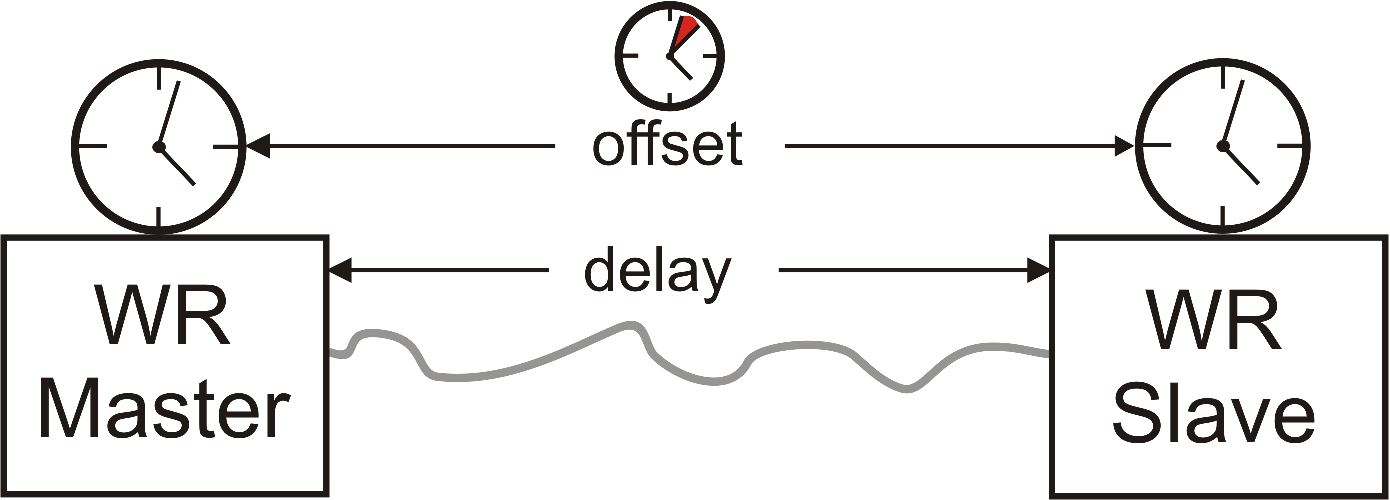
\includegraphics[height=3cm]{protocol/wrLink.ps}
  \end{center}

\end{frame}
%%%%%%%%%%%%%%%%%%%%%%%%%%%%%%%%%%%%%%%%%%%%%%%%%%%%%%%%%%%%%%%%%%%%%%%%%%%%%%%%%%%%%%%%%%%%%%%%%%%%
% \subsection{}
%%%%%%%%%%%%%%%%%%%%%%%%%%%%%%%%%%%%%%%%%%%%%%%%%%%%%%%%%%%%%%%%%%%%%%%%%%%%%%%%%%%%%%%%%%%%%%%%%%%%
\begin{frame}{Time Distribution in White Rabbit}

\center A White Rabbit Network
  \begin{center}
  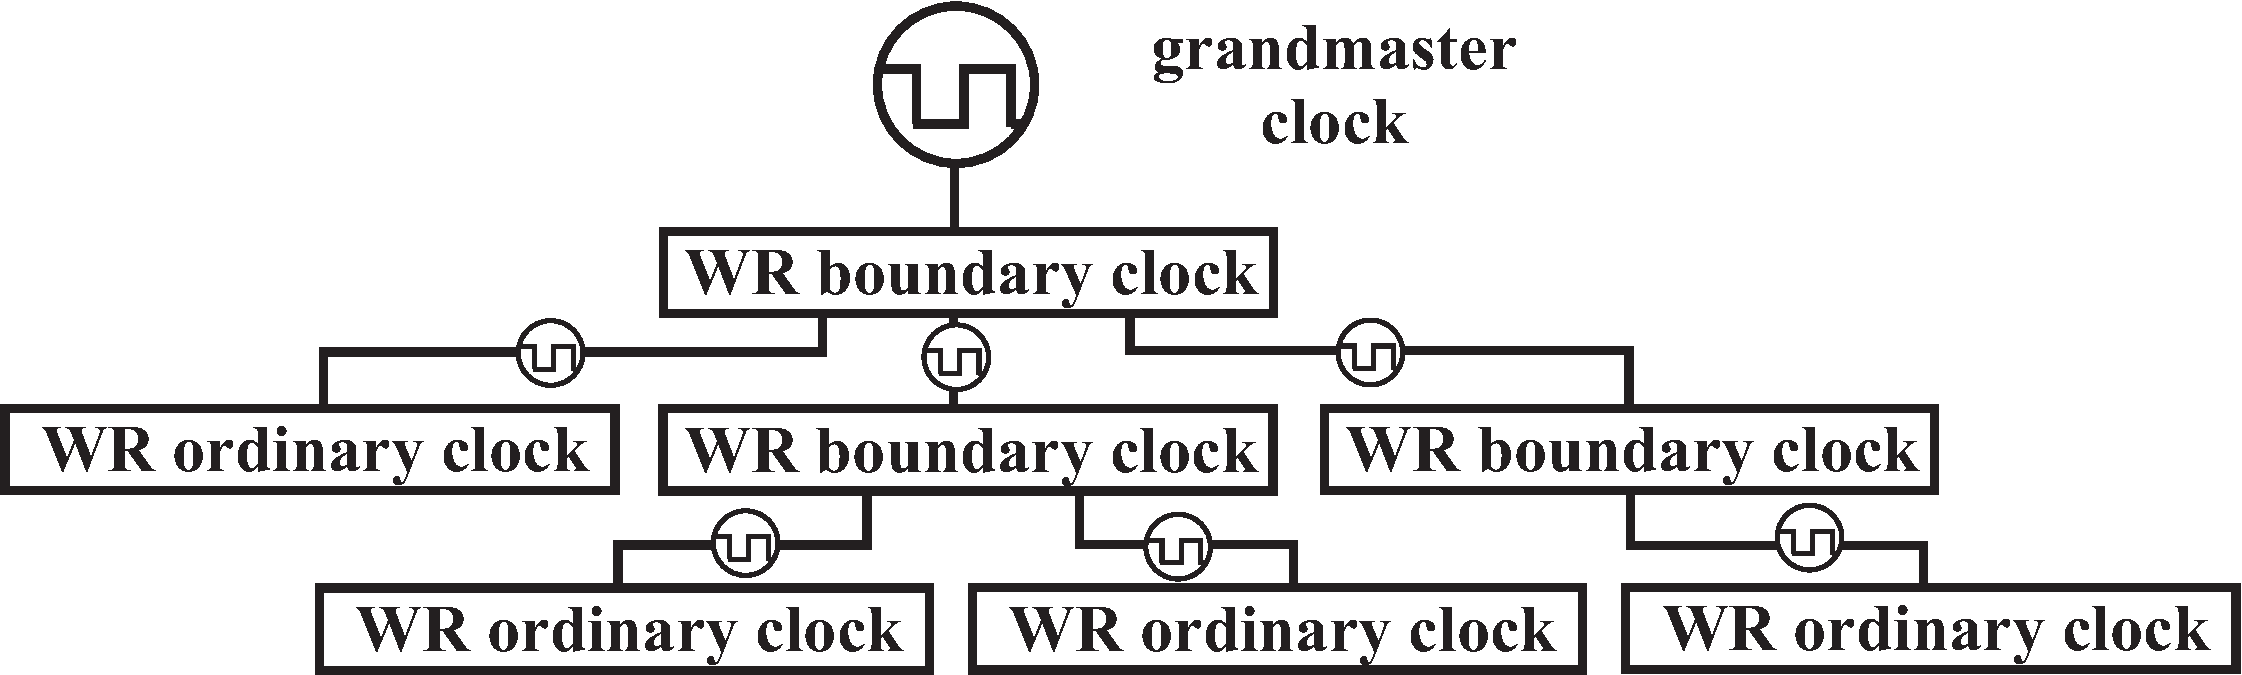
\includegraphics[width=11.5cm]{network/wrTopology.eps}
  \end{center}
\end{frame}
%%%%%%%%%%%%%%%%%%%%%%%%%%%%%%%%%%%%%%%%%%%%%%%%%%%%%%%%%%%%%%%%%%%%%%%%%%%%%%%%%%%%%%%%%%%%%%%%%%%%
\section{Why not standard PTP?}
\subsection{}
% %%%%%%%%%%%%%%%%%%%%%%%%%%%%%%%%%%%%%%%%%%%%%%%%%%%%%%%%%%%%%%%%%%%%%%%%%%%%%%%%%%%%%%%%%%%%%%%%%%%%
% \begin{frame}{PTP is OK but ...}
% % 
% %   \begin{itemize}
% %     \item Limited precision and resolution,
% %     \item Unknown physical link asymmetry,
% %     \item PTP-based syntonization vs. traffic load.
% %   \end{itemize}
% 
%   \resizebox{11cm}{!} 
%   {
%     \begin{tabular}{ r c l }
%       PTP-base		 	& $=>$ & traffic load  \\
%       syntonization	        &      &        \\
% 				&      &        \\
%       limited             	& $=>$ & limited accuracy \\
%       precision and resolution  &      &  \\
% 				&      &        \\
%       unknown                   &      &   \\
%       physical link asymmetry   & $=>$ & limited accuracy 	\\
% 				&      & \color{white}{DDTMD phase detection}			\\
% 				&      &        		\\
%       \multicolumn{3}{c}{\color{white}{WR extension to PTP ({\bf WRPTP}}) for } \\
%       \multicolumn{3}{c}{\color{white}{extra data exchange and logic}} \\
%     \end{tabular}
%   }
% 
% \end{frame}
%%%%%%%%%%%%%%%%%%%%%%%%%%%%%%%%%%%%%%%%%%%%%%%%%%%%%%%%%%%%%%%%%%%%%%%%%%%%%%%%%%%%%%%%%%%%%%%%%%%%
% \subsection{}
%%%%%%%%%%%%%%%%%%%%%%%%%%%%%%%%%%%%%%%%%%%%%%%%%%%%%%%%%%%%%%%%%%%%%%%%%%%%%%%%%%%%%%%%%%%%%%%%%%%%
%\begin{frame}{Addressing the issues}
\begin{frame}{PTP is OK but ...}

  \resizebox{11cm}{!} 
  {
    \begin{tabular}{ r c l }
  {\bf What are the issues...} 	& {\bf and}      & {\bf ... how we address them}  \\
				&     		 &        \\
      PTP-base		 	& \multirow{2}{*}{$\Rightarrow$}  & \multirow{2}{*}{SyncE }\\
      syntonization	        &      		 &        \\
				&      		 &        			\\
      limited             	&\multirow{2}{*}{$\Rightarrow$}  	 & SyncE \\
      precision and resolution  &      		 & DDTMD phase detection\\
				&    		 &        \\
			        &      		 & SyncE  \\
      unknown link asymmetry    & $\Rightarrow$  & DDTMD phase detection \\
				&      		 & WR Link Delay Model \\
				&      		 &        \\
      \multicolumn{3}{c}{WR extension to PTP ({\bf WRPTP}) for } \\
      \multicolumn{3}{c}{extra data exchange and logic} \\
    \end{tabular}
  }
\end{frame}
% %%%%%%%%%%%%%%%%%%%%%%%%%%%%%%%%%%%%%%%%%%%%%%%%%%%%%%%%%%%%%%%%%%%%%%%%%%%%%%%%%%%%%%%%%%%%%%%%%%%%
% \section{Technologies}
% \subsection{}
% %%%%%%%%%%%%%%%%%%%%%%%%%%%%%%%%%%%%%%%%%%%%%%%%%%%%%%%%%%%%%%%%%%%%%%%%%%%%%%%%%%%%%%%%%%%%%%%%%%%%
% \begin{frame}{SyncE syntonization}
% 
% {\it [(1)Steal an animation by Eva ?]} \\
% {\it [(2)Remove ?]}
% 
% \end{frame}
%%%%%%%%%%%%%%%%%%%%%%%%%%%%%%%%%%%%%%%%%%%%%%%%%%%%%%%%%%%%%%%%%%%%%%%%%%%%%%%%%%%%%%%%%%%%%%%%%%%%
% \subsection{}
%%%%%%%%%%%%%%%%%%%%%%%%%%%%%%%%%%%%%%%%%%%%%%%%%%%%%%%%%%%%%%%%%%%%%%%%%%%%%%%%%%%%%%%%%%%%%%%%%%%%
% \begin{frame}{DDMTD phase detection}
% 
% {\it[remove ?]}
% 
%   \begin{center}
%   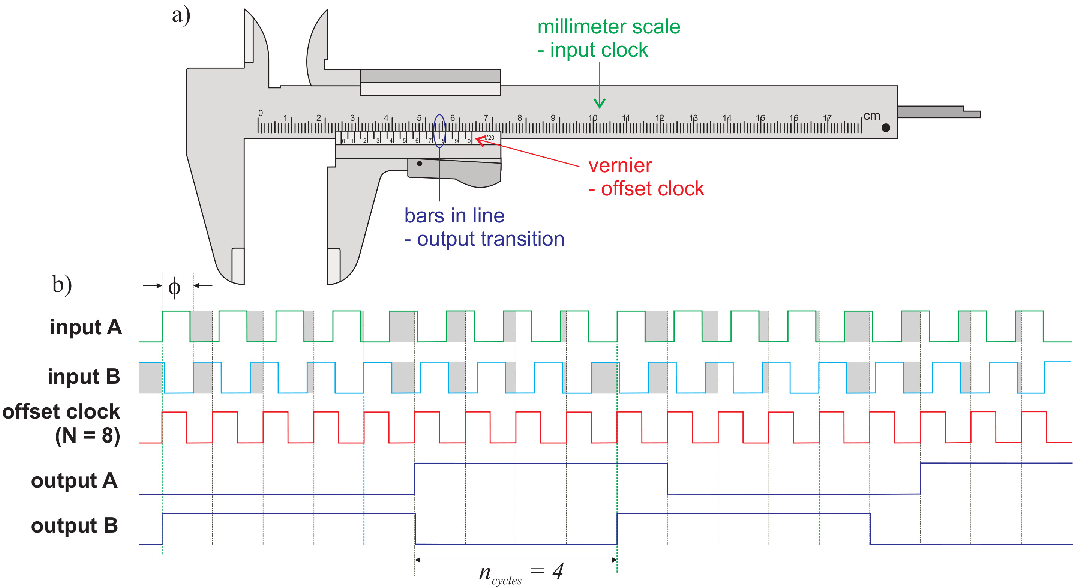
\includegraphics[width=11cm]{fig/dmtd_vernier.eps}
%   \end{center}
% 
% \end{frame}
%%%%%%%%%%%%%%%%%%%%%%%%%%%%%%%%%%%%%%%%%%%%%%%%%%%%%%%%%%%%%%%%%%%%%%%%%%%%%%%%%%%%%%%%%%%%%%%%%%%%
\section{Link Delay Model}
\subsection{}
%%%%%%%%%%%%%%%%%%%%%%%%%%%%%%%%%%%%%%%%%%%%%%%%%%%%%%%%%%%%%%%%%%%%%%%%%%%%%%%%%%%%%%%%%%%%%%%%%%%%
\begin{frame}{Link Delay Model}

  \begin{align}
    \nonumber delay_{ms} &= \Delta_{tx_m} + \delta_{ms} + \Delta_{rx_s} \\
    \nonumber delay_{sm} &= \Delta_{tx_s} + \delta_{sm} + \Delta_{rx_m}
  \end{align}

   \vspace{0.2cm}

  \begin{center}
  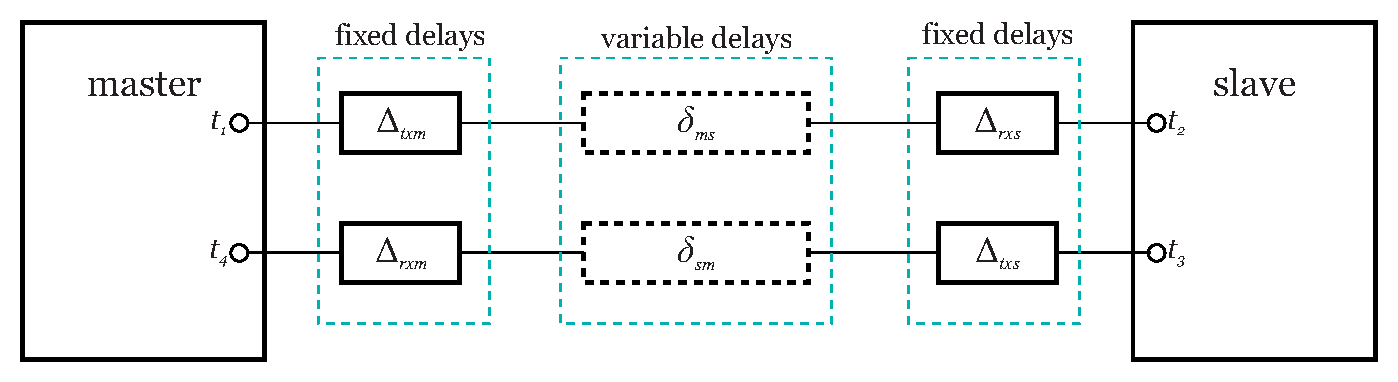
\includegraphics[height=2.5cm]{protocol/delaymodel.eps}
  \end{center}

\begin{columns}[c]
  \column{2.8in}

    \begin{center}
      \textbf{Relative Delay Coefficient ($\alpha$)} \\
      for 1000base-X over a Single-mode Optical Fibre
    \end{center}

  \column{1.5in}
    \begin{center}
      \begin{equation}
      \nonumber \delta_{ms} = (1 + \alpha) \, \delta_{sm}
      \end{equation}
    \end{center}
    \vspace{0.5cm}
\end{columns}
  

\end{frame}
%%%%%%%%%%%%%%%%%%%%%%%%%%%%%%%%%%%%%%%%%%%%%%%%%%%%%%%%%%%%%%%%%%%%%%%%%%%%%%%%%%%%%%%%%%%%%%%%%%%%
% \subsection{}
%%%%%%%%%%%%%%%%%%%%%%%%%%%%%%%%%%%%%%%%%%%%%%%%%%%%%%%%%%%%%%%%%%%%%%%%%%%%%%%%%%%%%%%%%%%%%%%%%%%%
\begin{frame}{Link Delay Model: fiber optic solution}

  \begin{center}
  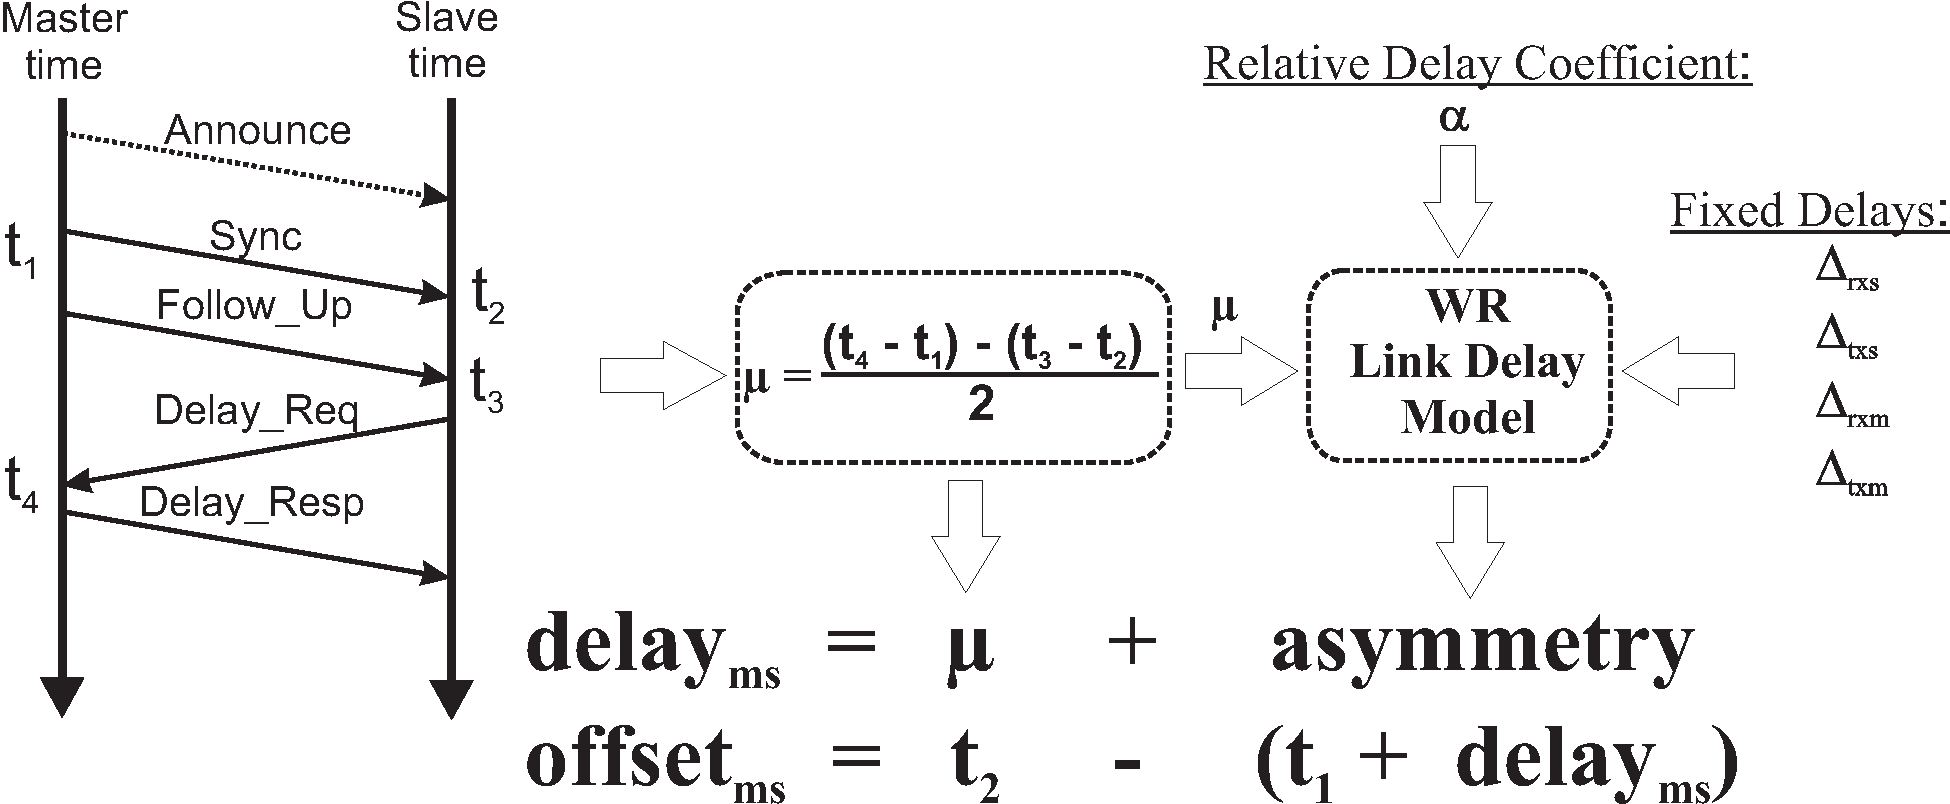
\includegraphics[height=4cm]{protocol/wrLinkModel.eps}
  \end{center}

  \begin{columns}[c]
  \column{1.5in}

    \begin{center}
      \textbf{Solution for Ethernet over a Single-mode Optical Fiber}
    \end{center}    

  \column{2.7in}

    \begin{equation}
      \nonumber asymmetry = \Delta_{tx_m} + \Delta_{rx_s} - \frac{\Delta - \alpha \mu + \alpha \Delta}{2 + \alpha}
    \end{equation}

  \end{columns}

\end{frame}
% %%%%%%%%%%%%%%%%%%%%%%%%%%%%%%%%%%%%%%%%%%%%%%%%%%%%%%%%%%%%%%%%%%%%%%%%%%%%%%%%%%%%%%%%%%%%%%%%%%%%
% \section{}
% \subsection{}
% %%%%%%%%%%%%%%%%%%%%%%%%%%%%%%%%%%%%%%%%%%%%%%%%%%%%%%%%%%%%%%%%%%%%%%%%%%%%%%%%%%%%%%%%%%%%%%%%%%%%
% \begin{frame}{Overview of White Rabbit Distribution}
% 
% fill in
% 
% \end{frame}
%%%%%%%%%%%%%%%%%%%%%%%%%%%%%%%%%%%%%%%%%%%%%%%%%%%%%%%%%%%%%%%%%%%%%%%%%%%%%%%%%%%%%%%%%%%%%%%%%%%%
\section{H/W for WR}
\subsection{}
%%%%%%%%%%%%%%%%%%%%%%%%%%%%%%%%%%%%%%%%%%%%%%%%%%%%%%%%%%%%%%%%%%%%%%%%%%%%%%%%%%%%%%%%%%%%%%%%%%%%
% \begin{frame}{HW4WR}
% 
%   \begin{itemize}
%     \item Fine Delay Measurement,
%     \item Clock Recovery System,
%     \item Fixed Delays Measurement.
%   \end{itemize}
% 
% 
% \end{frame}
%%%%%%%%%%%%%%%%%%%%%%%%%%%%%%%%%%%%%%%%%%%%%%%%%%%%%%%%%%%%%%%%%%%%%%%%%%%%%%%%%%%%%%%%%%%%%%%%%%%%
% \subsection{}
%%%%%%%%%%%%%%%%%%%%%%%%%%%%%%%%%%%%%%%%%%%%%%%%%%%%%%%%%%%%%%%%%%%%%%%%%%%%%%%%%%%%%%%%%%%%%%%%%%%%
\setbeamertemplate{background}{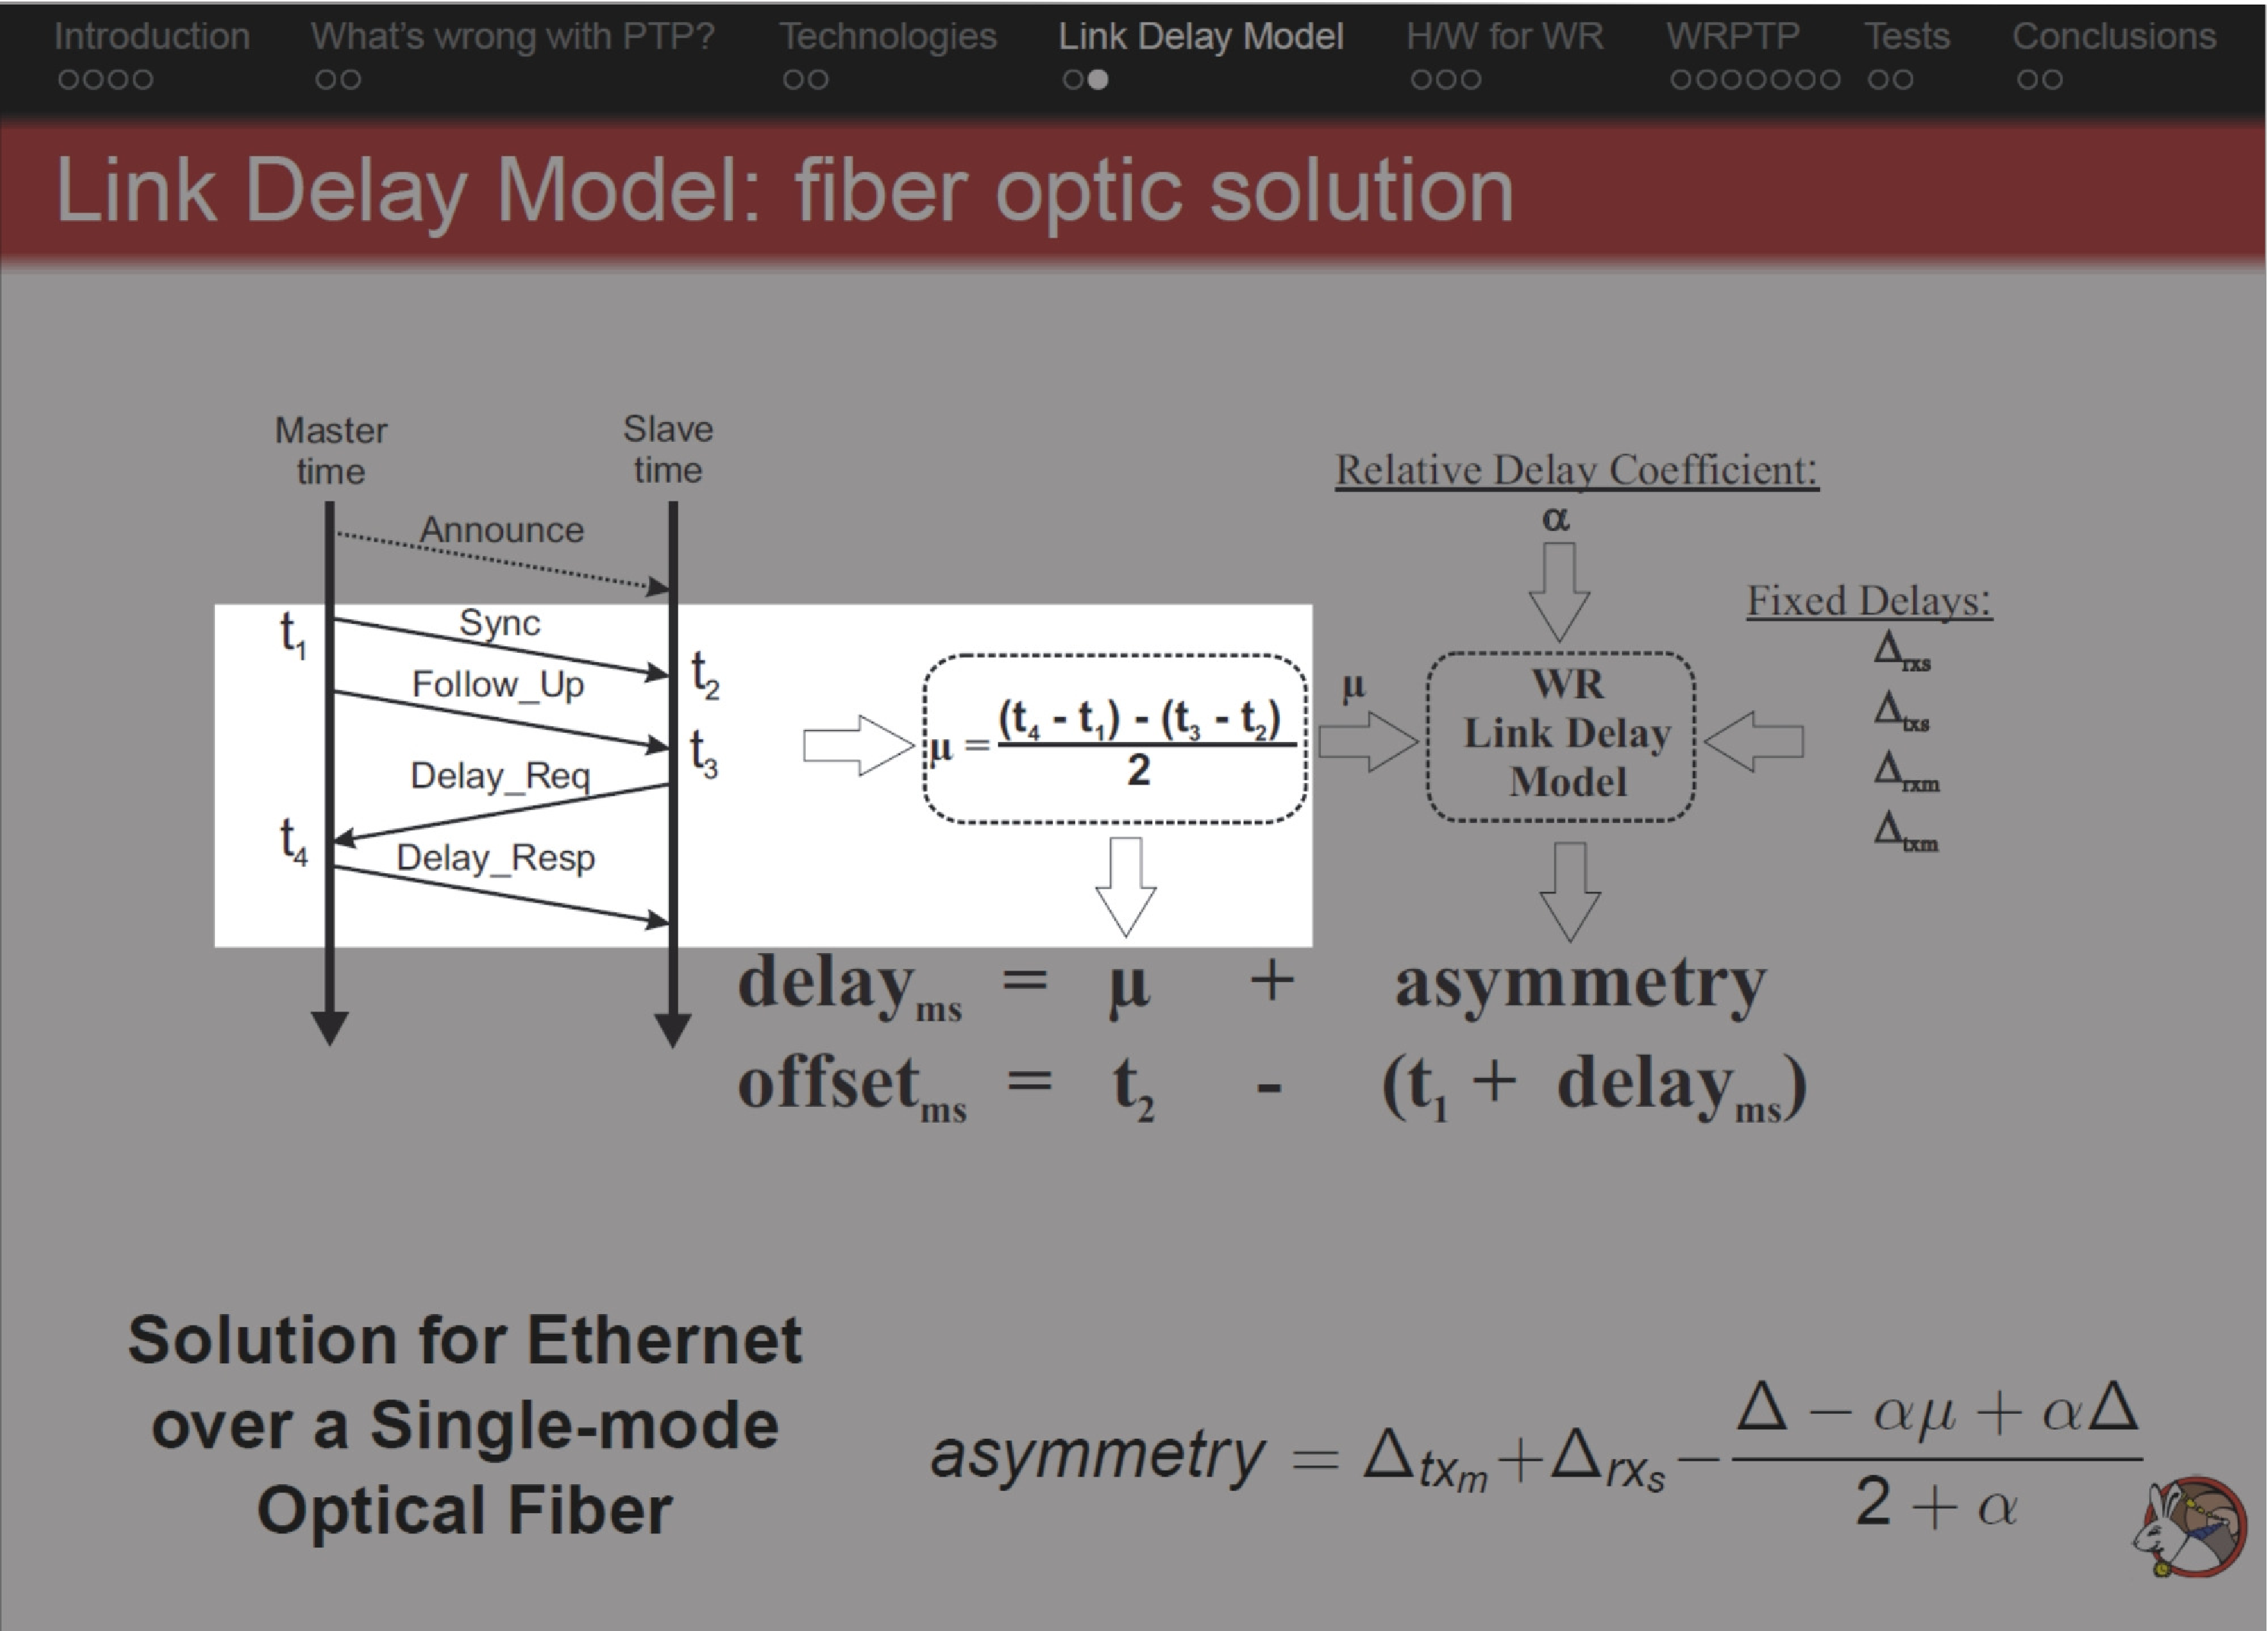
\includegraphics[width=\paperwidth]{protocol/wrLinkModel-fdm2.ps}}
\logo{}
\begin{frame}{Fine Delay Measurement}

%background

\end{frame}
\setbeamertemplate{background}{} 
\logo{\pgfuseimage{wr-logo}}
%%%%%%%%%%%%%%%%%%%%%%%%%%%%%%%%%%%%%%%%%%%%%%%%%%%%%%%%%%%%%%%%%%%%%%%%%%%%%%%%%%%%%%%%%%%%%%%%%%%%
%\subsection{}
%%%%%%%%%%%%%%%%%%%%%%%%%%%%%%%%%%%%%%%%%%%%%%%%%%%%%%%%%%%%%%%%%%%%%%%%%%%%%%%%%%%%%%%%%%%%%%%%%%%%
\begin{frame}{Fine Delay Measurement}

  \begin{center}
  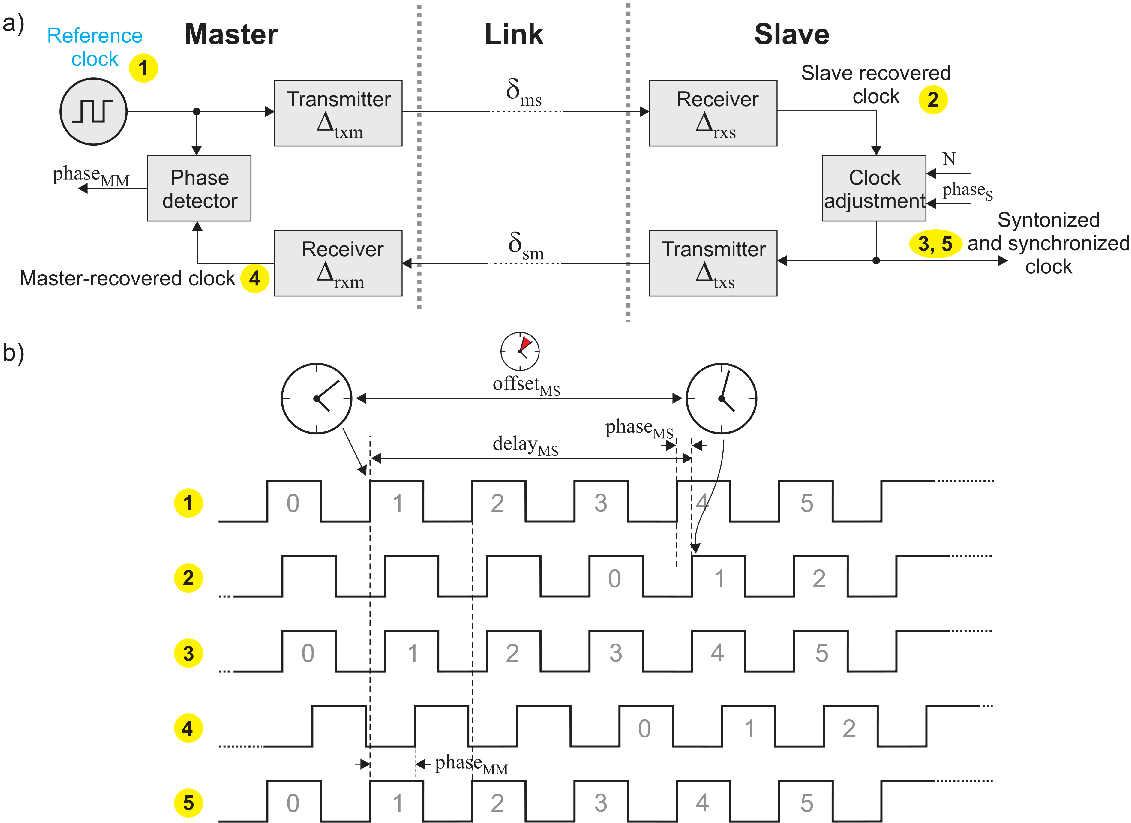
\includegraphics[width=10.0cm]{protocol/link_model.eps}
  \end{center}

\end{frame}

%%%%%%%%%%%%%%%%%%%%%%%%%%%%%%%%%%%%%%%%%%%%%%%%%%%%%%%%%%%%%%%%%%%%%%%%%%%%%%%%%%%%%%%%%%%%%%%%%%%%
%\subsection{}
%%%%%%%%%%%%%%%%%%%%%%%%%%%%%%%%%%%%%%%%%%%%%%%%%%%%%%%%%%%%%%%%%%%%%%%%%%%%%%%%%%%%%%%%%%%%%%%%%%%%
\setbeamertemplate{background}{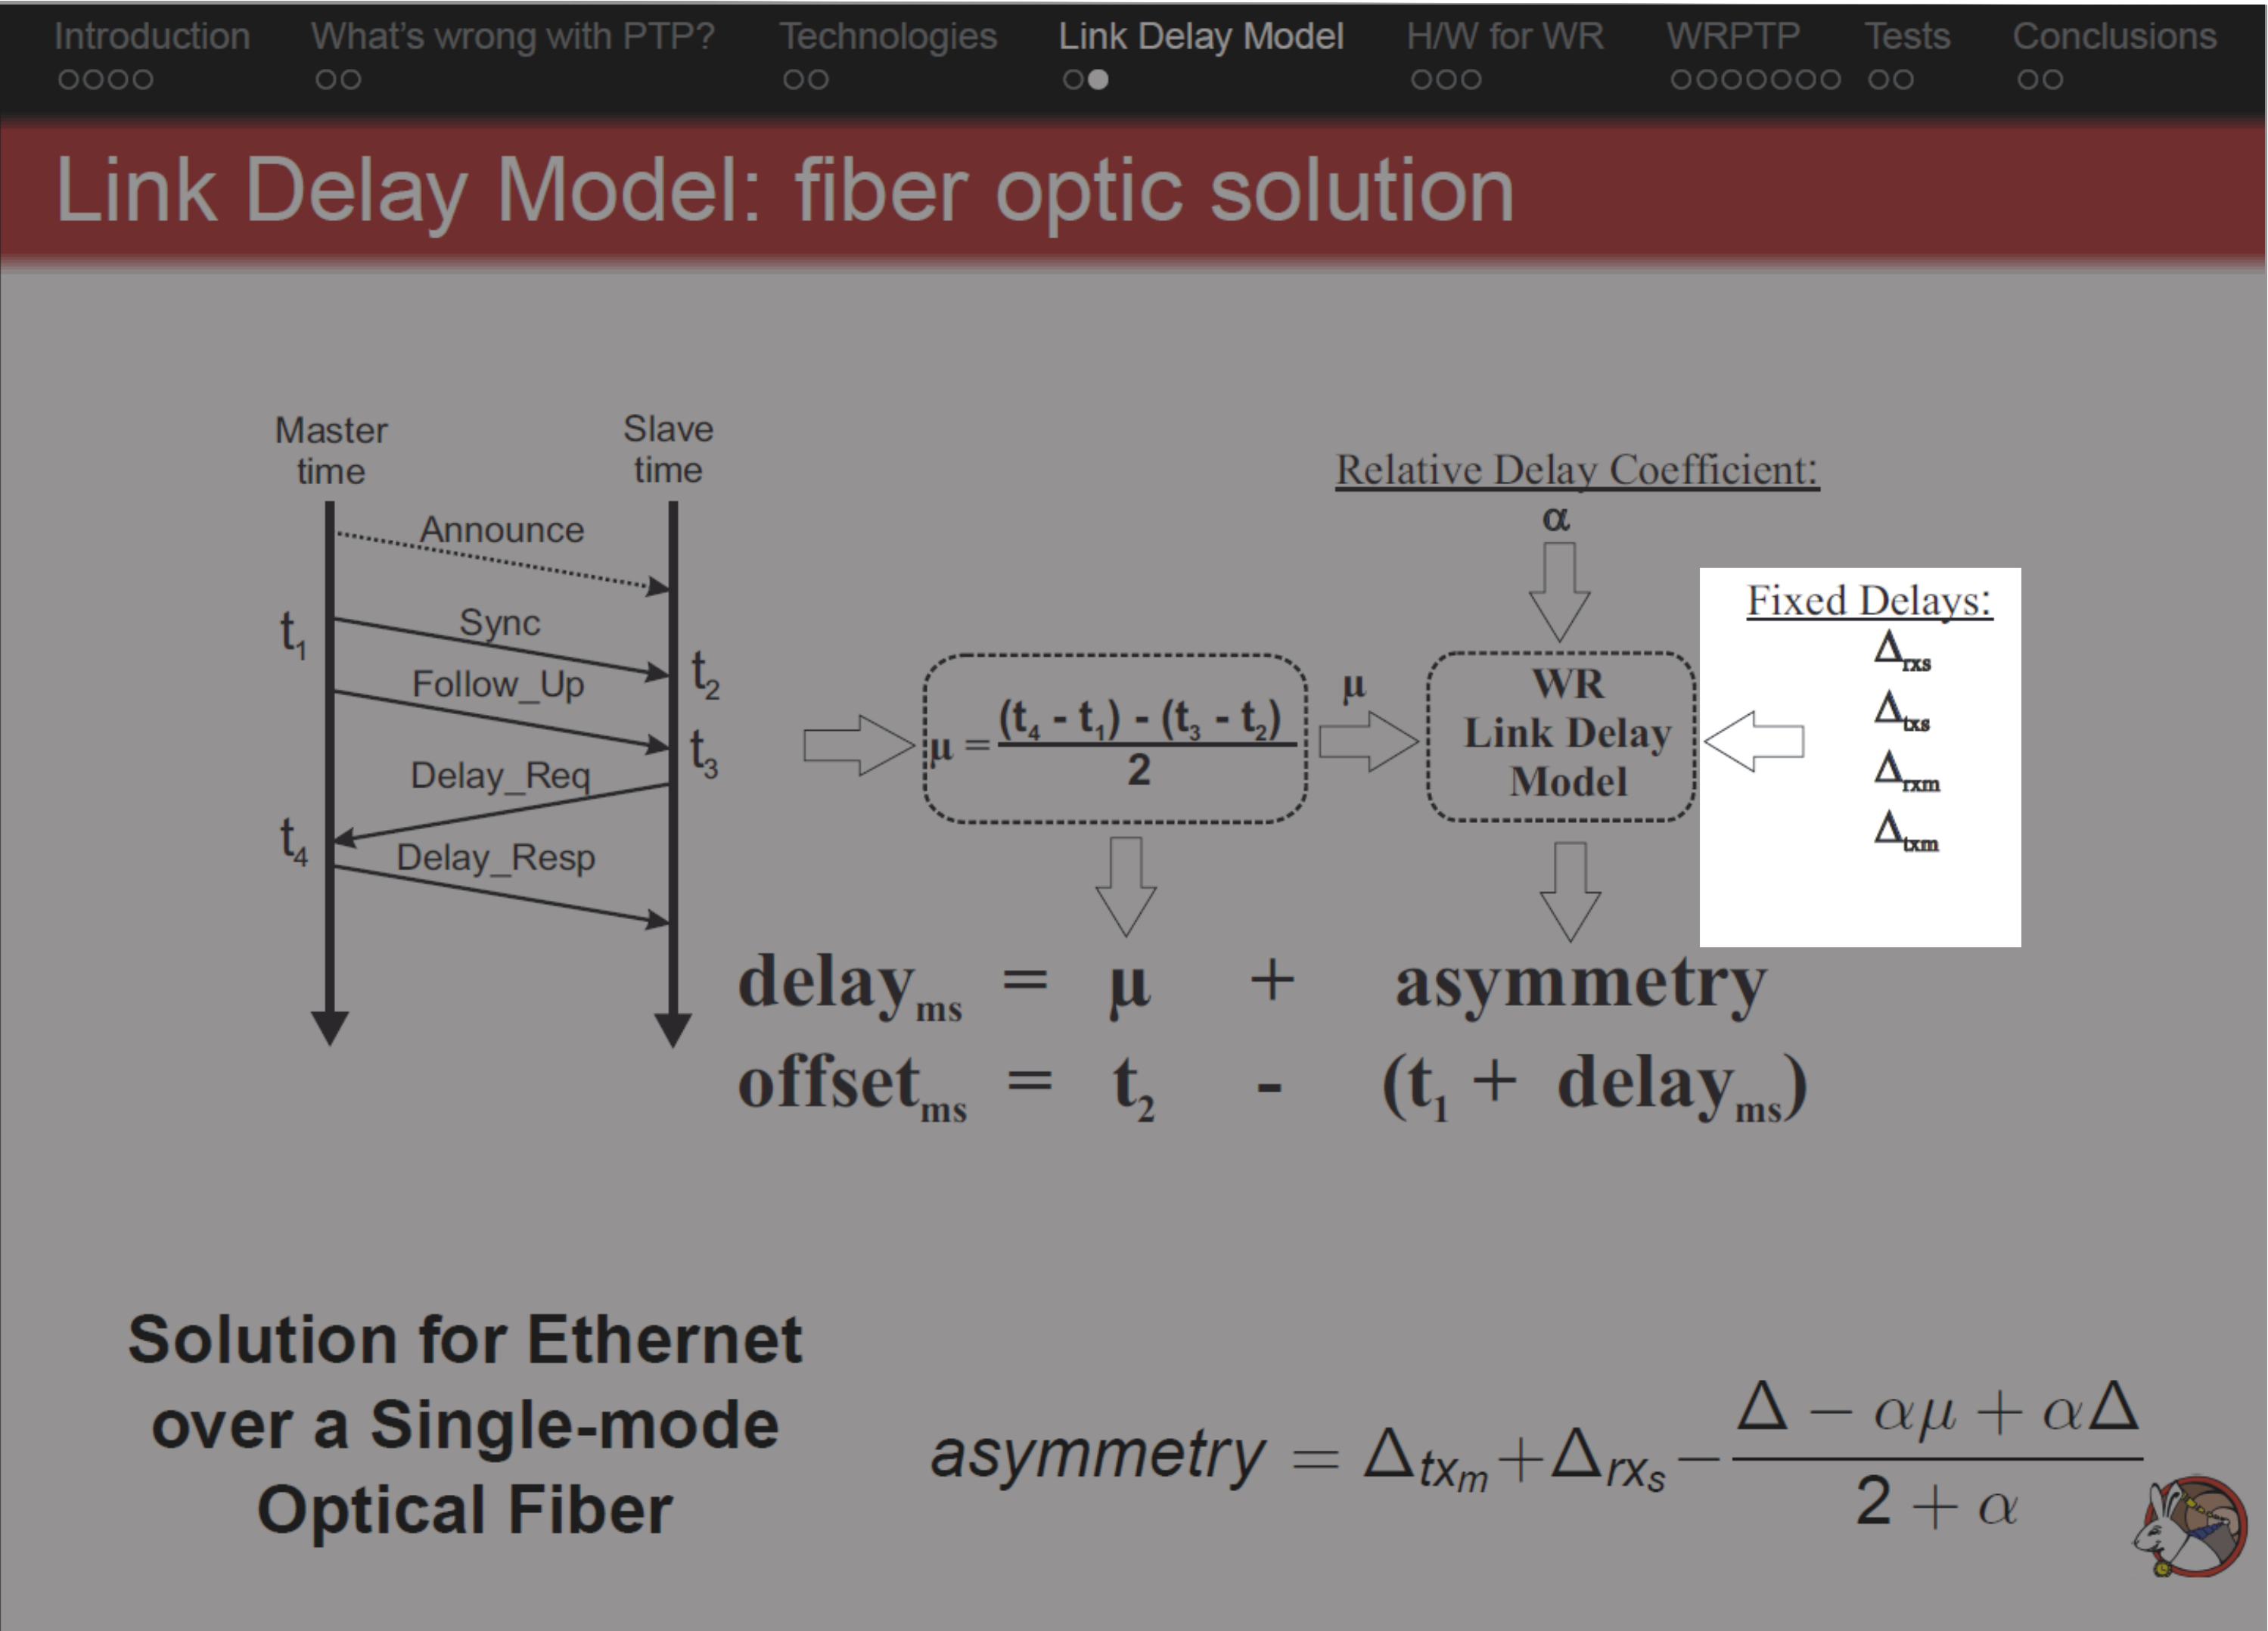
\includegraphics[width=\paperwidth]{protocol/wrLinkModel-fd.ps}}
\logo{}
\begin{frame}{Fixed Delays Measurement}

%background

\end{frame}
\setbeamertemplate{background}{} 
\logo{\pgfuseimage{wr-logo}}
%%%%%%%%%%%%%%%%%%%%%%%%%%%%%%%%%%%%%%%%%%%%%%%%%%%%%%%%%%%%%%%%%%%%%%%%%%%%%%%%%%%%%%%%%%%%%%%%%%%%
%\subsection{}
%%%%%%%%%%%%%%%%%%%%%%%%%%%%%%%%%%%%%%%%%%%%%%%%%%%%%%%%%%%%%%%%%%%%%%%%%%%%%%%%%%%%%%%%%%%%%%%%%%%%
\begin{frame}{Fixed Delays Measurement}

  \begin{center}
  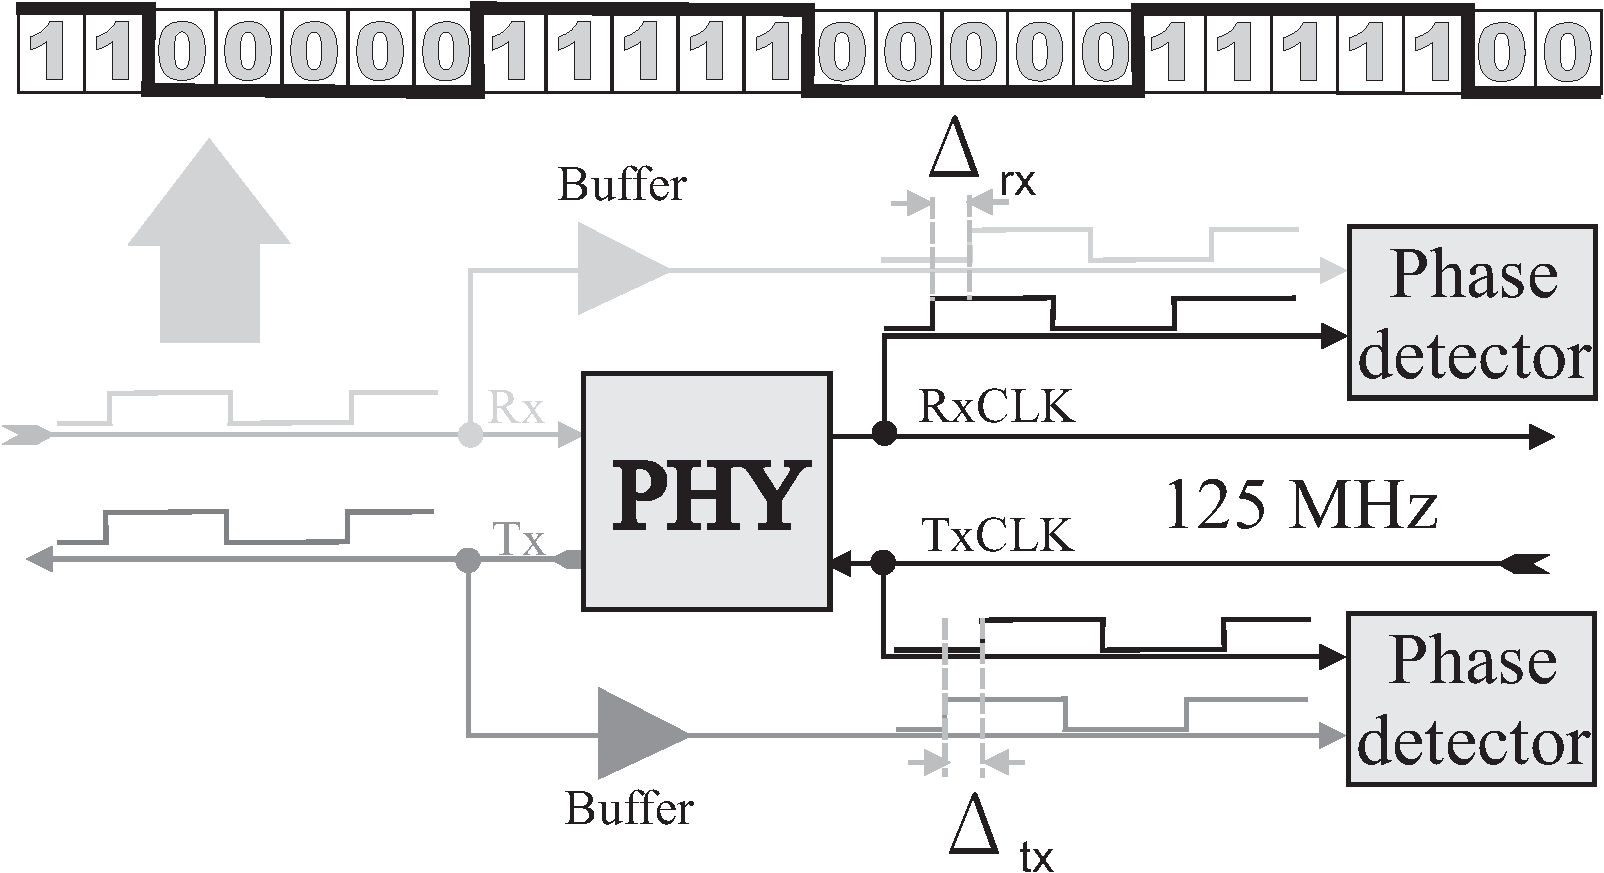
\includegraphics[width=10.0cm]{misc/calibration.eps}
  \end{center}

\end{frame}
% %%%%%%%%%%%%%%%%%%%%%%%%%%%%%%%%%%%%%%%%%%%%%%%%%%%%%%%%%%%%%%%%%%%%%%%%%%%%%%%%%%%%%%%%%%%%%%%%%%%%
% \subsection{}
% %%%%%%%%%%%%%%%%%%%%%%%%%%%%%%%%%%%%%%%%%%%%%%%%%%%%%%%%%%%%%%%%%%%%%%%%%%%%%%%%%%%%%%%%%%%%%%%%%%%%
% \begin{frame}{Clock Recovery System}
% 
% {\it [problem with a presentation flow]}
% 
%   \begin{center}
%   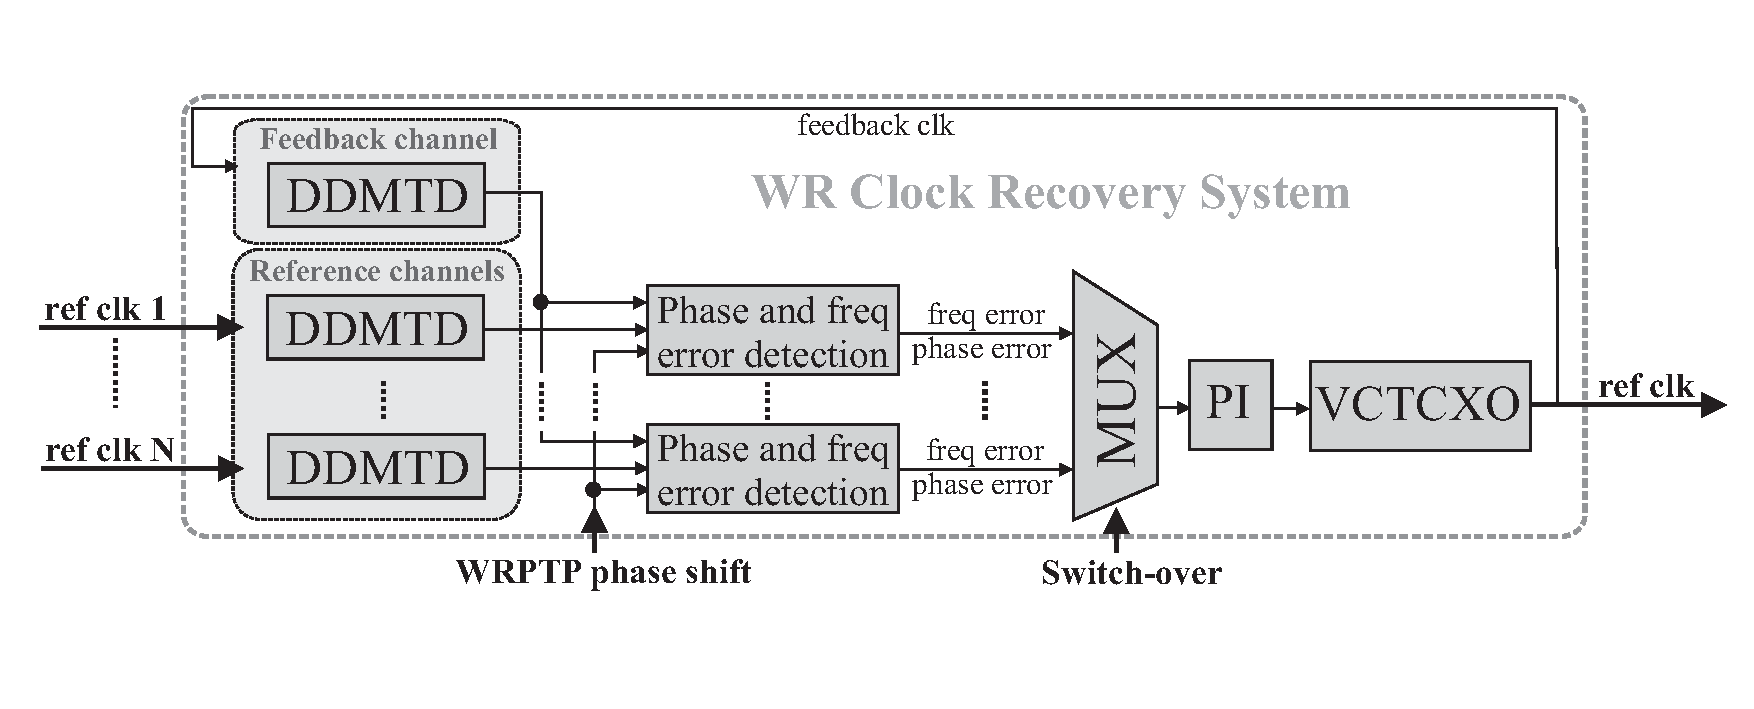
\includegraphics[width=11.5cm]{fig/wrCRS.eps}
%   \end{center}
% 
% \end{frame}
%%%%%%%%%%%%%%%%%%%%%%%%%%%%%%%%%%%%%%%%%%%%%%%%%%%%%%%%%%%%%%%%%%%%%%%%%%%%%%%%%%%%%%%%%%%%%%%%%%%%
\section{WRPTP}
\subsection{}
%%%%%%%%%%%%%%%%%%%%%%%%%%%%%%%%%%%%%%%%%%%%%%%%%%%%%%%%%%%%%%%%%%%%%%%%%%%%%%%%%%%%%%%%%%%%%%%%%%%%
\begin{frame}{White Rabbit extension to PTP (WRPTP)}

  \begin{itemize}
    \item WR-peers recognition,
    \item Calibration,
    \item Exchange of WR-data,
    \item Support of redundancy.
  \end{itemize}

\end{frame}
% we need to exchange some extra WR data in order to recognize WR peers (syncE),
% the exchange of data is also needed to perform calibration, where also some extra logic is needed
% and finaly to exchange the WR parameters. Finally, the support of time-source redundancy by 
% the standard PTP is not enough for WR, so we needed to change this as well
%%%%%%%%%%%%%%%%%%%%%%%%%%%%%%%%%%%%%%%%%%%%%%%%%%%%%%%%%%%%%%%%%%%%%%%%%%%%%%%%%%%%%%%%%%%%%%%%%%%%
% \subsection{}
%%%%%%%%%%%%%%%%%%%%%%%%%%%%%%%%%%%%%%%%%%%%%%%%%%%%%%%%%%%%%%%%%%%%%%%%%%%%%%%%%%%%%%%%%%%%%%%%%%%%
% \begin{frame}{Exchange of WR-data}
% 
%   \begin{itemize}
%     \item WR Type-Length-Value (WR TLV):
%       \begin{itemize}
% 	\item tlvType=ORGANIZATION\_EXTENSION
% 	\item OrganizationID=CERN's OUI
%       \end{itemize}
%     \vspace{0.5cm}
%     \item WR data exchange by:
%       \begin{itemize}
% 	\item suffixing Announce Messages
% 	\item creating WR Signaling Messages
%       \end{itemize}
%   \end{itemize}
% 
% \end{frame}
% %%%%%%%%%%%%%%%%%%%%%%%%%%%%%%%%%%%%%%%%%%%%%%%%%%%%%%%%%%%%%%%%%%%%%%%%%%%%%%%%%%%%%%%%%%%%%%%%%%%%
% % \subsection{}
% %%%%%%%%%%%%%%%%%%%%%%%%%%%%%%%%%%%%%%%%%%%%%%%%%%%%%%%%%%%%%%%%%%%%%%%%%%%%%%%%%%%%%%%%%%%%%%%%%%%%
% \begin{frame}{WR-peers recognision}
% 
%   \begin{columns}[c]
%   \column{.5\textwidth} 
% 
%     \begin{center}
%     \includegraphics[width=5.5cm]{fig/WR-peer_recognision-1.eps}
%     \end{center}
% 
%   \column{.5\textwidth}
% 
%     \begin{center}
%     \includegraphics[width=5.5cm]{fig/WR-peer_recognision-2.eps}
%     \end{center}
% 
%   \end{columns}
% 
% \end{frame}
%%%%%%%%%%%%%%%%%%%%%%%%%%%%%%%%%%%%%%%%%%%%%%%%%%%%%%%%%%%%%%%%%%%%%%%%%%%%%%%%%%%%%%%%%%%%%%%%%%%%
% \subsection{}
%%%%%%%%%%%%%%%%%%%%%%%%%%%%%%%%%%%%%%%%%%%%%%%%%%%%%%%%%%%%%%%%%%%%%%%%%%%%%%%%%%%%%%%%%%%%%%%%%%%%
\begin{frame}{Exchange of WR-data}

  \begin{columns}[c]
  \column{.5\textwidth} 

    \begin{center}
    \includegraphics[width=5.5cm]{protocol/WR-peer_recognision-1.eps}
    \end{center}

  \column{.5\textwidth}

    \begin{center}
    \includegraphics[width=5.5cm]{protocol/WR-peer_recognision-2.eps}
    \end{center}

  \end{columns}

\end{frame}
%%%%%%%%%%%%%%%%%%%%%%%%%%%%%%%%%%%%%%%%%%%%%%%%%%%%%%%%%%%%%%%%%%%%%%%%%%%%%%%%%%%%%%%%%%%%%%%%%%%%
% \subsection{}
%%%%%%%%%%%%%%%%%%%%%%%%%%%%%%%%%%%%%%%%%%%%%%%%%%%%%%%%%%%%%%%%%%%%%%%%%%%%%%%%%%%%%%%%%%%%%%%%%%%%
\begin{frame}{WR Link Setup }

  \begin{columns}[c]
  \column{.5\textwidth} 

      \begin{center}
      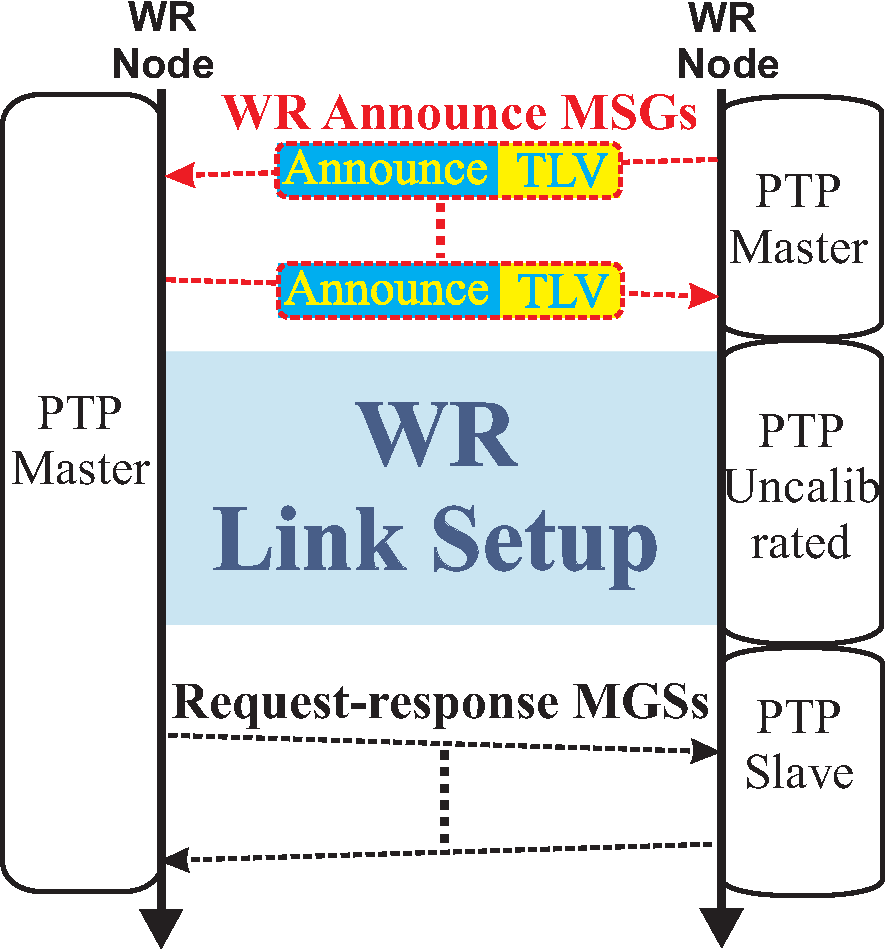
\includegraphics[width=5.5cm]{protocol/wrLinkSetup.eps}
      \end{center}


  \column{.5\textwidth} 

      \begin{itemize}
	\item Frequency locking
	\item Calibration
	\item Exchange of WR-parameters
	\item WR Finite State Machine (FSM)
	\item WR Signaling Messages
      \end{itemize}

  \end{columns}

\end{frame}
%%%%%%%%%%%%%%%%%%%%%%%%%%%%%%%%%%%%%%%%%%%%%%%%%%%%%%%%%%%%%%%%%%%%%%%%%%%%%%%%%%%%%%%%%%%%%%%%%%%%
% \subsection{}
%%%%%%%%%%%%%%%%%%%%%%%%%%%%%%%%%%%%%%%%%%%%%%%%%%%%%%%%%%%%%%%%%%%%%%%%%%%%%%%%%%%%%%%%%%%%%%%%%%%%
% \begin{frame}{WR Link Setup}
% 
%       \begin{center}
%       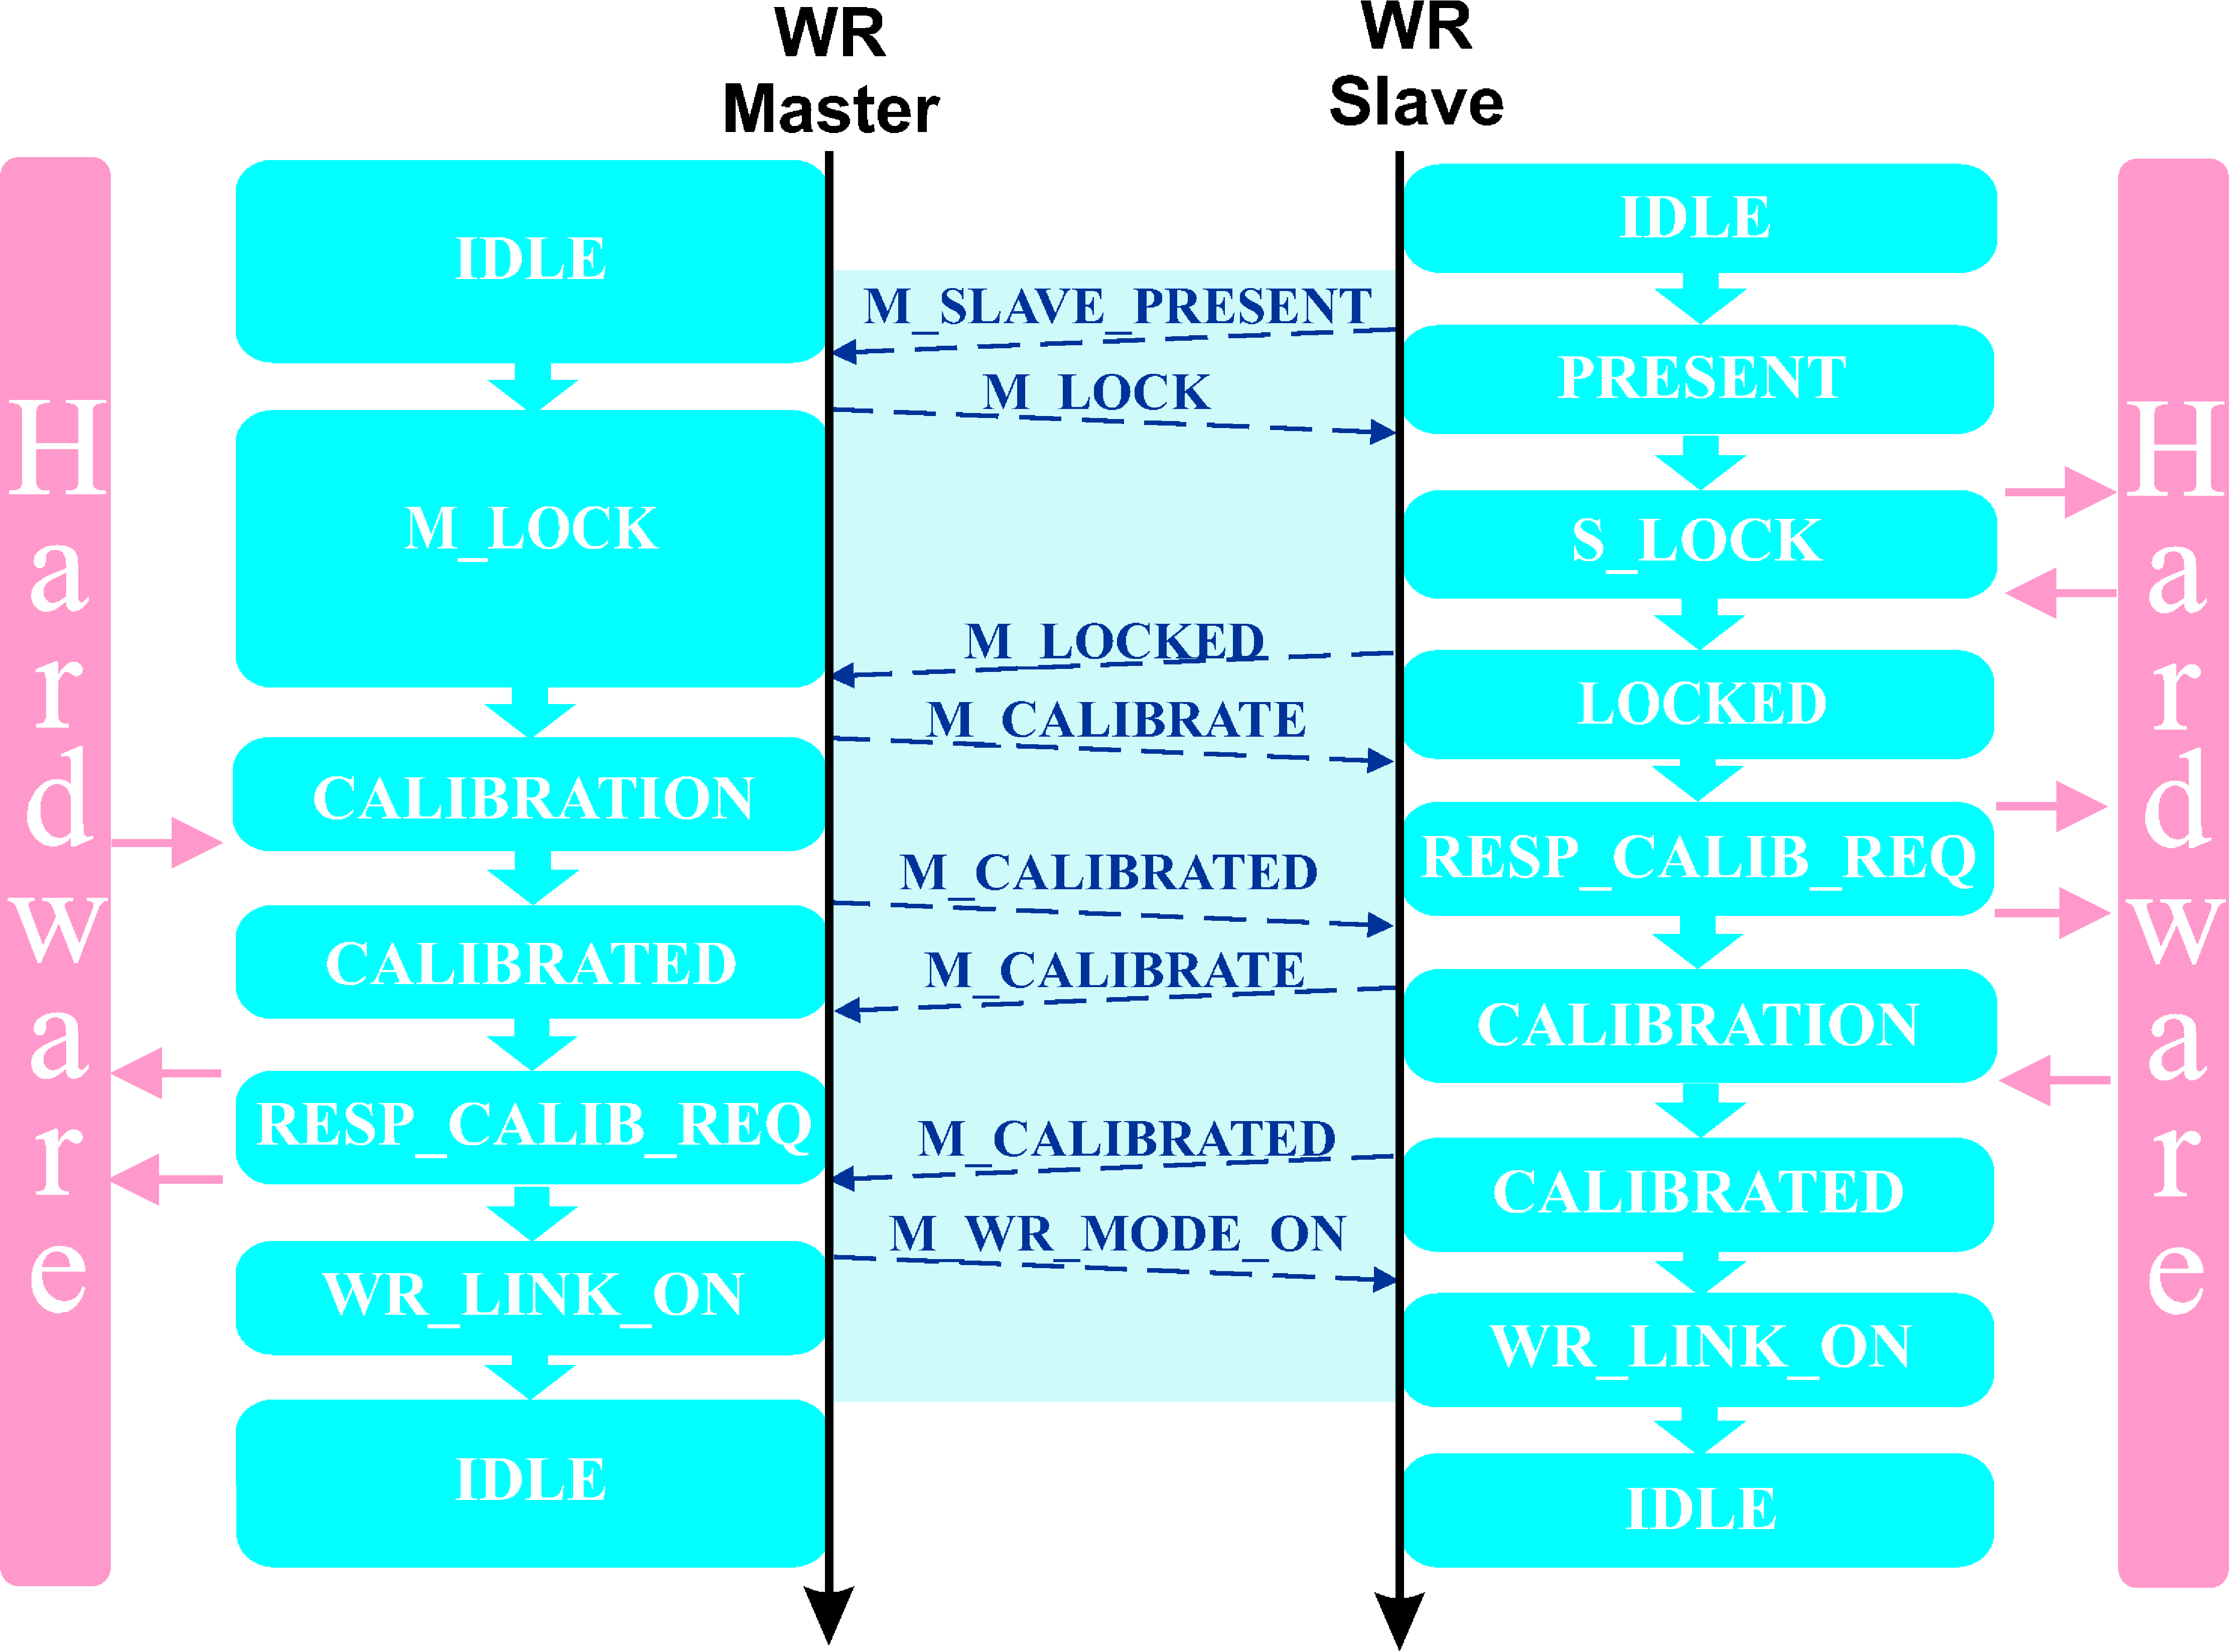
\includegraphics[width=9.5cm]{fig/wrLinkSetupFSM.eps}
%       \end{center}
% 
% \end{frame}
%%%%%%%%%%%%%%%%%%%%%%%%%%%%%%%%%%%%%%%%%%%%%%%%%%%%%%%%%%%%%%%%%%%%%%%%%%%%%%%%%%%%%%%%%%%%%%%%%%%%
% \subsection{}
%%%%%%%%%%%%%%%%%%%%%%%%%%%%%%%%%%%%%%%%%%%%%%%%%%%%%%%%%%%%%%%%%%%%%%%%%%%%%%%%%%%%%%%%%%%%%%%%%%%%
% \begin{frame}{Redundancy: BMC}
% 
% \begin{columns}[c]
% \column{.6\textwidth} 
%     \begin{itemize}
% 	\item disjoint logic trees for multiple \textit{best} clocks,
% 	\item redundancy not optimal for the continuity of the synchronization,
% 	\item no more than one PTP SLAVE port in a single Boundary Clock.
%       \end{itemize}
% {\it[correct spelling of GPS in fig]}
% \column{.4\textwidth}
%     \begin{center}
%     \includegraphics[height=7.0cm]{fig/BMC.eps}
%      \end{center}
% \end{columns}
% 
% 
% \end{frame}
%%%%%%%%%%%%%%%%%%%%%%%%%%%%%%%%%%%%%%%%%%%%%%%%%%%%%%%%%%%%%%%%%%%%%%%%%%%%%%%%%%%%%%%%%%%%%%%%%%%%
% \subsection{}
%%%%%%%%%%%%%%%%%%%%%%%%%%%%%%%%%%%%%%%%%%%%%%%%%%%%%%%%%%%%%%%%%%%%%%%%%%%%%%%%%%%%%%%%%%%%%%%%%%%%
% \begin{frame}{Redundancy: modified BMC}
% 
% \begin{columns}[c]
% \column{.6\textwidth}
% 
%     \begin{block}{Modified BMC}
%     ... forces PTP\_SLAVE state instead of PTP\_PASSIVE for clockClass $>$ 127
%     \end{block}
% 
%     \begin{itemize}
% 	\item Many PTP SLAVE ports in a single Boundary Clock,
% 	\item Active PTP SLAVE port used to synchronize and syntonize local clock.
% 	\item Modifies State Decision Algorithm.
% 	\item New Data Fields update. 
%       \end{itemize}
% {\it[correct spelling of GPS in fig]}
% \column{.4\textwidth}
%     \begin{center}
%     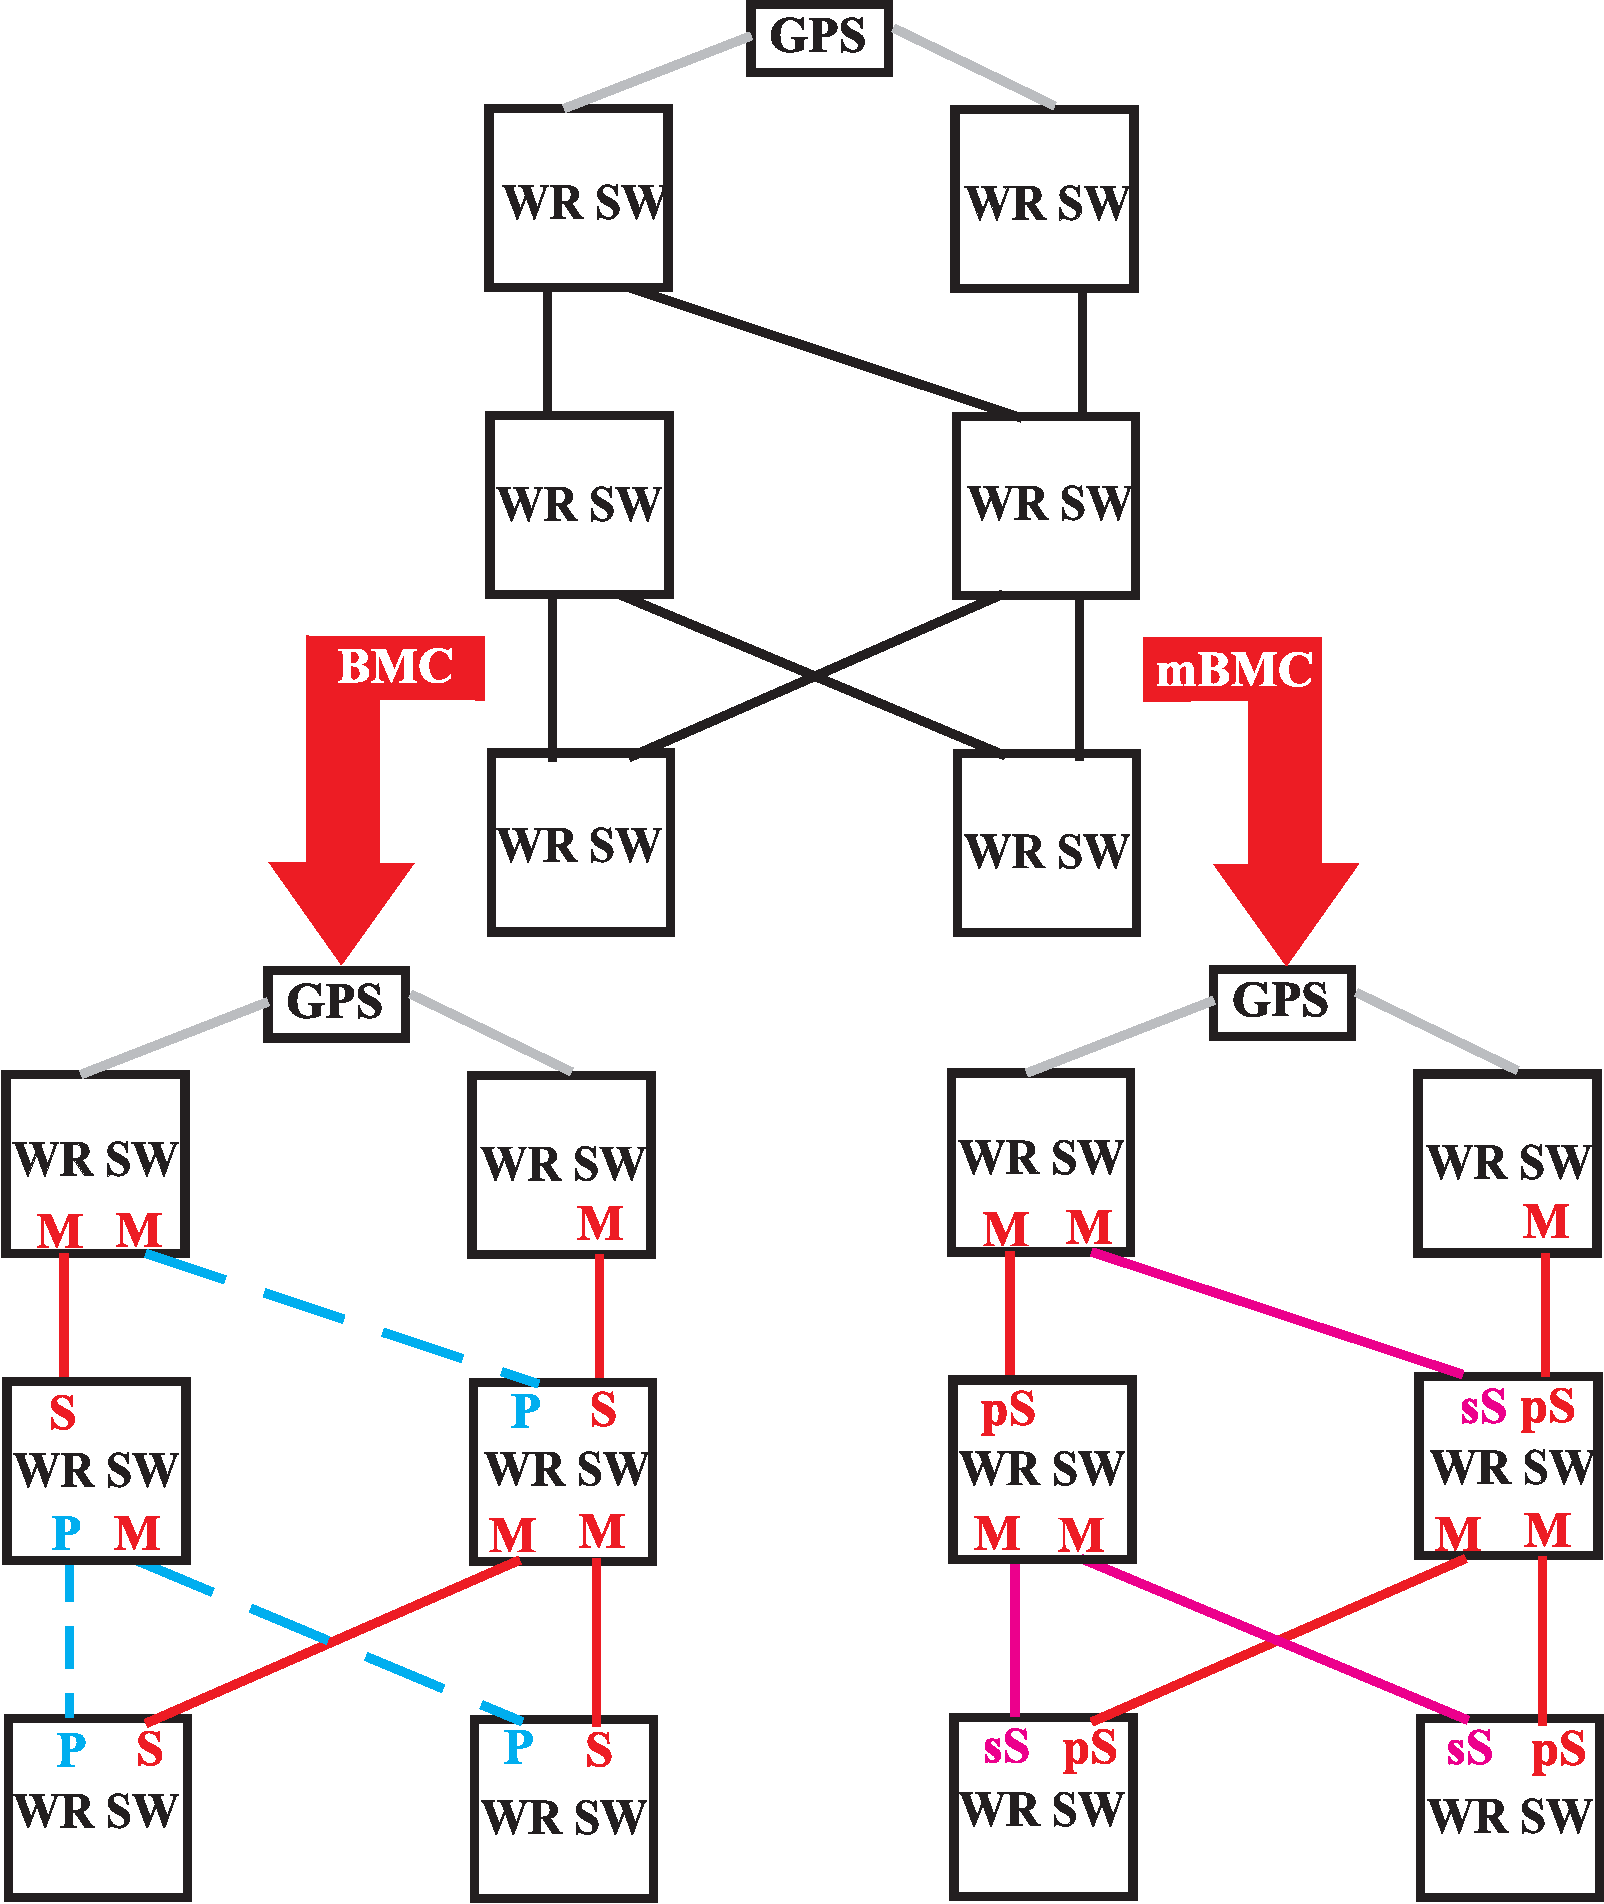
\includegraphics[height=7.0cm]{fig/mBMCvsBMC.eps}
%     \end{center}
% \end{columns}
% 
% \end{frame}
%%%%%%%%%%%%%%%%%%%%%%%%%%%%%%%%%%%%%%%%%%%%%%%%%%%%%%%%%%%%%%%%%%%%%%%%%%%%%%%%%%%%%%%%%%%%%%%%%%%%
% \section{H/W for WR}
% \subsection{H/W for WR}
%%%%%%%%%%%%%%%%%%%%%%%%%%%%%%%%%%%%%%%%%%%%%%%%%%%%%%%%%%%%%%%%%%%%%%%%%%%%%%%%%%%%%%%%%%%%%%%%%%%%
\begin{frame}{Clock Recovery System and modified BMC}

%{\it [problem with a presentation flow]}

  \begin{center}
  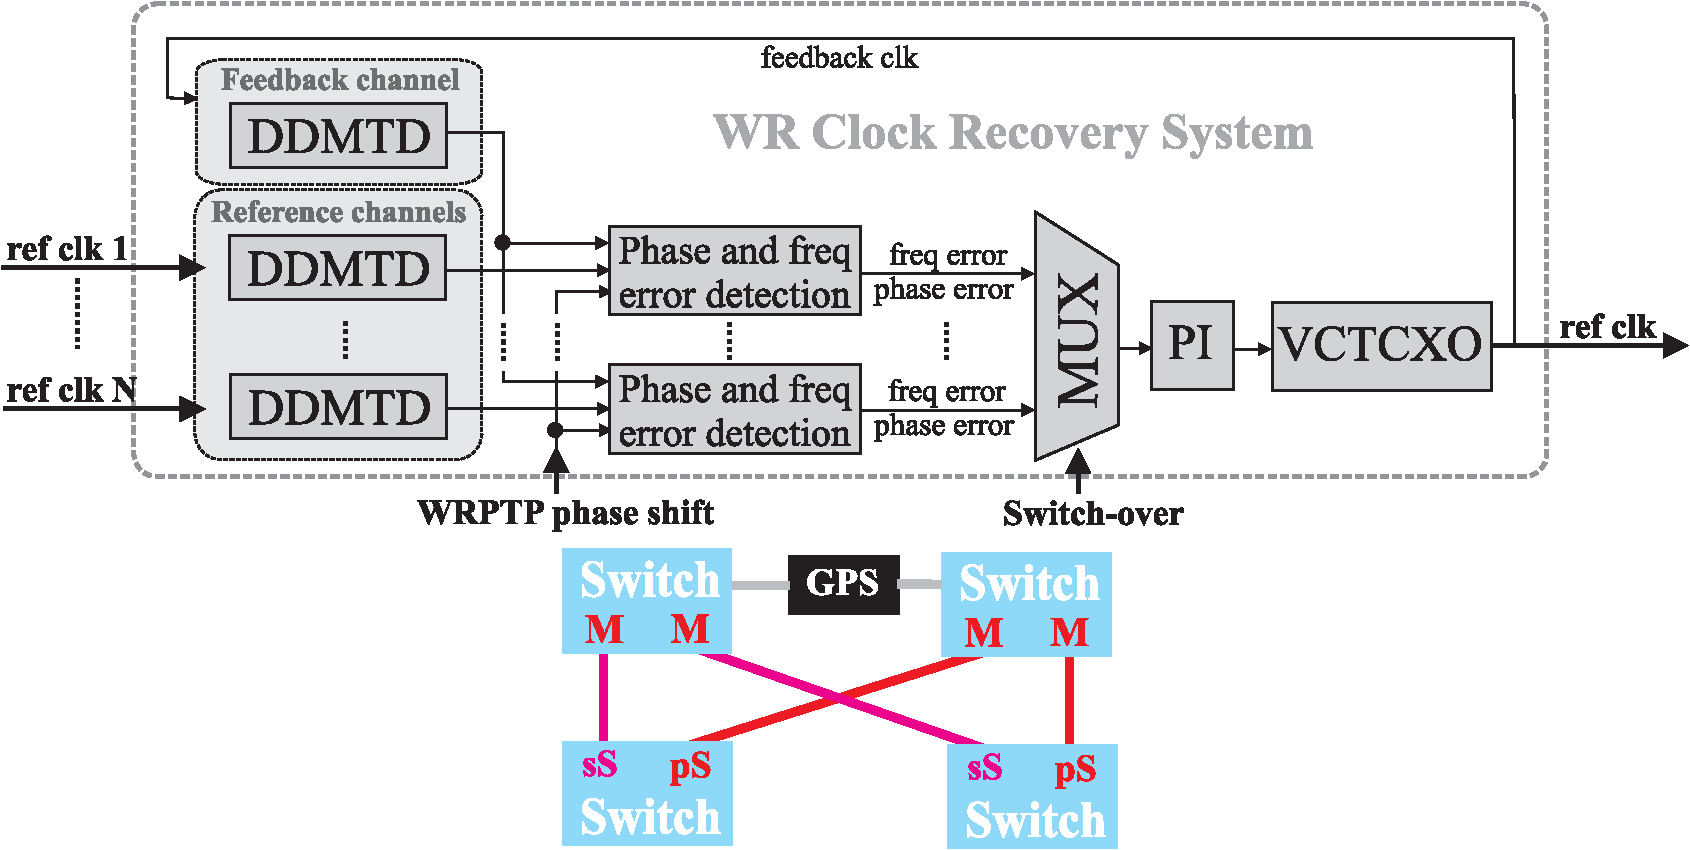
\includegraphics[width=11.8cm]{protocol/wrCRS_plus_mBMC.eps}
  \end{center}

\end{frame}
%%%%%%%%%%%%%%%%%%%%%%%%%%%%%%%%%%%%%%%%%%%%%%%%%%%%%%%%%%%%%%%%%%%%%%%%%%%%%%%%%%%%%%%%%%%%%%%%%%%%
\section{Status}
\subsection{}
%%%%%%%%%%%%%%%%%%%%%%%%%%%%%%%%%%%%%%%%%%%%%%%%%%%%%%%%%%%%%%%%%%%%%%%%%%%%%%%%%%%%%%%%%%%%%%%%%%%%
\begin{frame}{Test bed}

    \begin{center}
    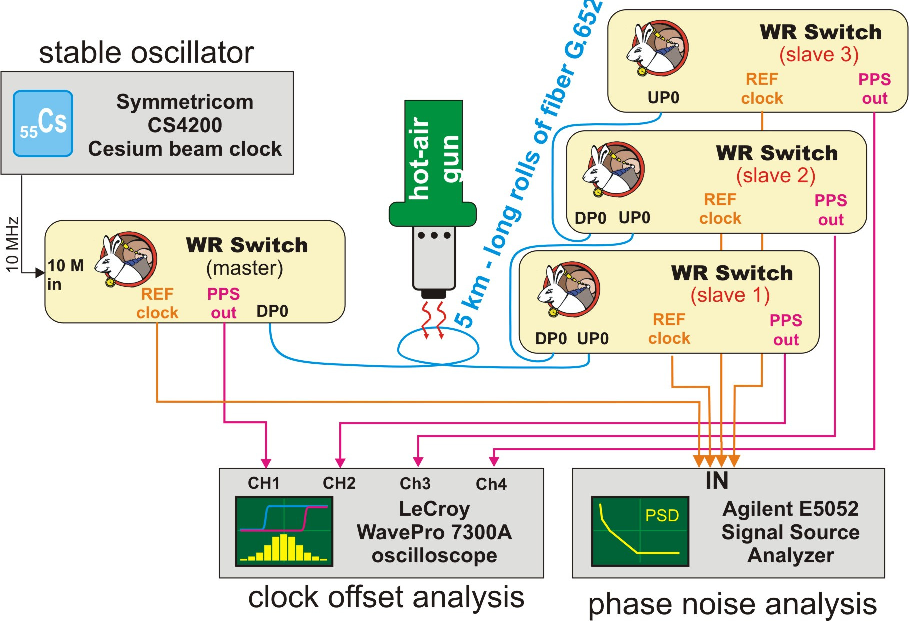
\includegraphics[height=7.0cm]{measurements/measSystem.ps}
    \end{center}

\end{frame}
%%%%%%%%%%%%%%%%%%%%%%%%%%%%%%%%%%%%%%%%%%%%%%%%%%%%%%%%%%%%%%%%%%%%%%%%%%%%%%%%%%%%%%%%%%%%%%%%%%%%
% \subsection{}
%%%%%%%%%%%%%%%%%%%%%%%%%%%%%%%%%%%%%%%%%%%%%%%%%%%%%%%%%%%%%%%%%%%%%%%%%%%%%%%%%%%%%%%%%%%%%%%%%%%%
\begin{frame}{Test results}

    \begin{center}
    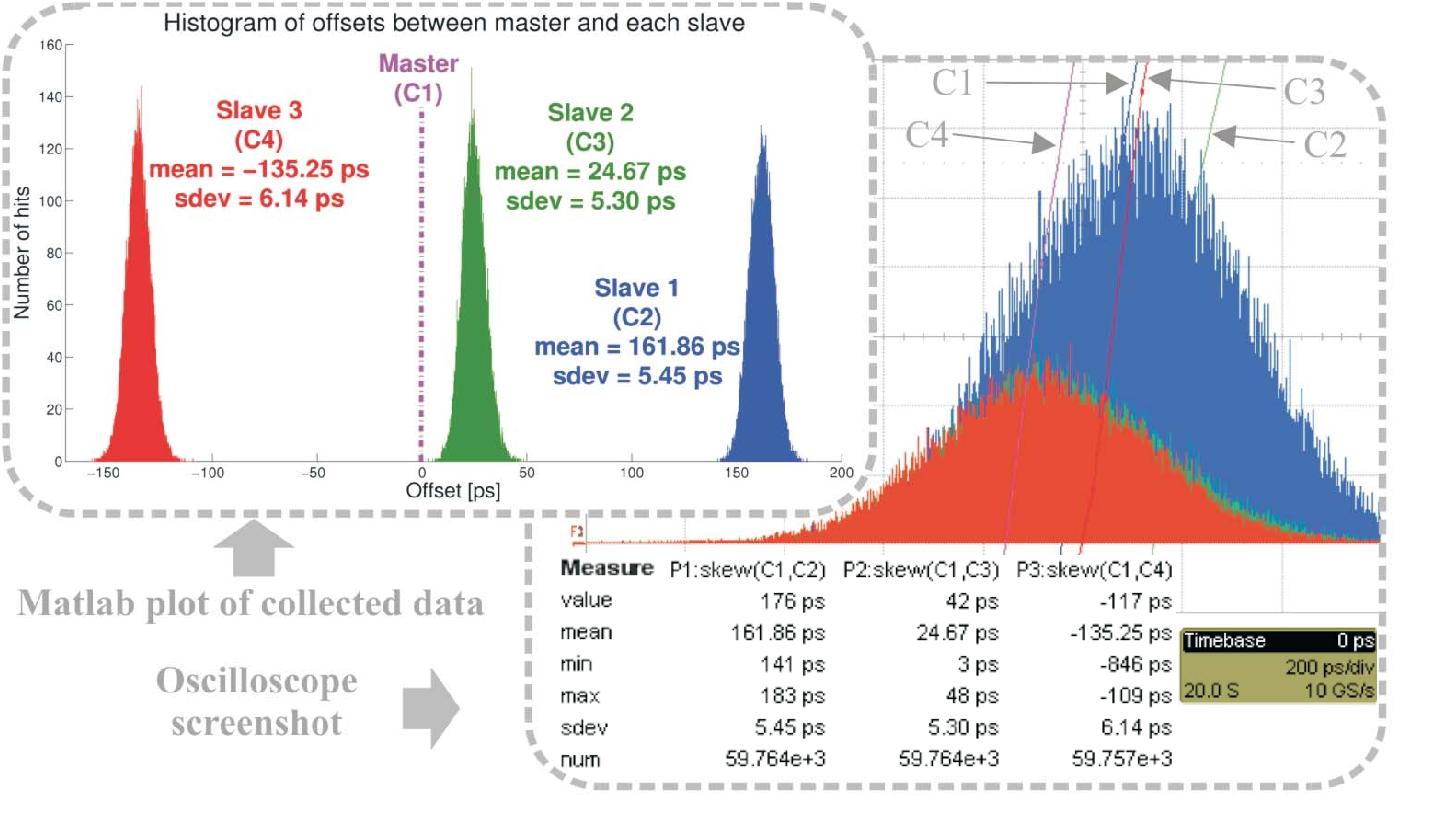
\includegraphics[height=6.0cm]{measurements/measResults-new.eps}
    \end{center}


\end{frame}
%%%%%%%%%%%%%%%%%%%%%%%%%%%%%%%%%%%%%%%%%%%%%%%%%%%%%%%%%%%%%%%%%%%%%%%%%%%%%%%%%%%%%%%%%%%%%%%%%%%%
% \subsection{}
%%%%%%%%%%%%%%%%%%%%%%%%%%%%%%%%%%%%%%%%%%%%%%%%%%%%%%%%%%%%%%%%%%%%%%%%%%%%%%%%%%%%%%%%%%%%%%%%%%%%
\begin{frame}{White Rabbit Switch (V2)}

    \begin{center}
    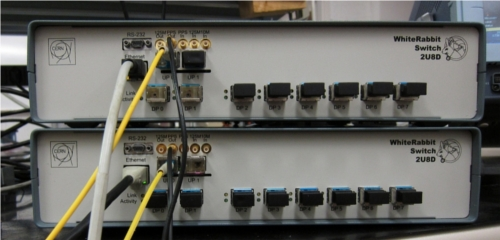
\includegraphics[width=8.0cm]{switch/old_switches2.ps}
    \end{center}

	\begin{itemize}
	\item Central element of WR network
	\item Fully custom design, designed from scratch
	\item 10 1000Base-LX ports
	\item capable of driving 10 km of SM fiber
%	\item 200 ps synchronization accuracy
	\end{itemize}




\end{frame}
%%%%%%%%%%%%%%%%%%%%%%%%%%%%%%%%%%%%%%%%%%%%%%%%%%%%%%%%%%%%%%%%%%%%%%%%%%%%%%%%%%%%%%%%%%%%%%%%%%%%
% \subsection{}
%%%%%%%%%%%%%%%%%%%%%%%%%%%%%%%%%%%%%%%%%%%%%%%%%%%%%%%%%%%%%%%%%%%%%%%%%%%%%%%%%%%%%%%%%%%%%%%%%%%%
\begin{frame}{WR-compliant Hardware Kit}

    \begin{center}
    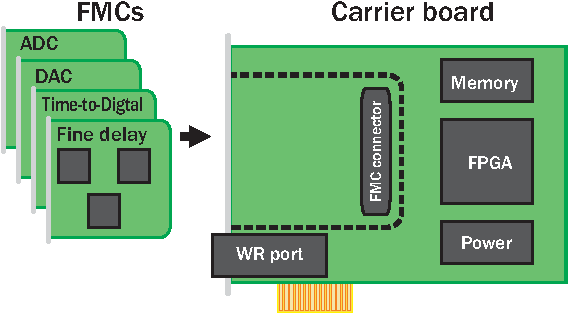
\includegraphics[width=6cm]{node/shw_kit.ps}
    \end{center}

  \begin{columns}[c]
    \column{.01\textwidth}
    \column{.98\textwidth}

	\begin{block}{Co-HT FMC-based Hardware Kit:}
	  \begin{itemize}
	  \item FMCs (FPGA Mezzanine Cards) with ADCs, DACs, TDCs, fine delays, digital I/O
	  \item Carrier boards in PCI-Express, VME and uTCA formats
	  \item All carriers are equipped with a White Rabbit port
	  \end{itemize}
	\end{block}

    \column{.01\textwidth}
  \end{columns}


\end{frame}
%%%%%%%%%%%%%%%%%%%%%%%%%%%%%%%%%%%%%%%%%%%%%%%%%%%%%%%%%%%%%%%%%%%%%%%%%%%%%%%%%%%%%%%%%%%%%%%%%%%%
\section{Conclusions}
\subsection{}
%%%%%%%%%%%%%%%%%%%%%%%%%%%%%%%%%%%%%%%%%%%%%%%%%%%%%%%%%%%%%%%%%%%%%%%%%%%%%%%%%%%%%%%%%%%%%%%%%%%%
\begin{frame}{Conclusions}

    \begin{itemize}
	\item Promising results
	\item Robust synchronization:
	  \begin{itemize}
	    \item high precision - rock solid synchronization
	    \item support of seamless switchover 
	  \end{itemize}
	\item Benefits from compatibility with standards:
	  \begin{itemize}
	    \item wide support
	    \item commercial feasibility
	    \item hybrid networks
	    \item general-purpose solution
	  \end{itemize}
	\item Great interest from many institutes and companies	
      \end{itemize}


\end{frame}
%%%%%%%%%%%%%%%%%%%%%%%%%%%%%%%%%%%%%%%%%%%%%%%%%%%%%%%%%%%%%%%%%%%%%%%%%%%%%%%%%%%%%%%%%%%%%%%%%%%%
\section{}
%\subsection{}
%%%%%%%%%%%%%%%%%%%%%%%%%%%%%%%%%%%%%%%%%%%%%%%%%%%%%%%%%%%%%%%%%%%%%%%%%%%%%%%%%%%%%%%%%%%%%%%%%%%%
\begin{frame}{thank you}

    \begin{center}
    Any questions ?
    \end{center}

    
    \begin{center}
%    \includegraphics[height=4.0cm]{fig/white_rabbit_by_kyoht.ps}
    \includegraphics[height=4.0cm]{logo/WRlogo.ps}
    \end{center}

\end{frame}
%%%%%%%%%%%%%%%%%%%%%%%%%%%%%%%%%%%%%%%%%%%%%%%%%%%%%%%%%%%%%%%%%%%%%%%%%%%%%%%%%%%%%%%%%%%%%%%%%%%%



\end{document}
